
\begin{abstract}
\textbf{Background:} A diabetes diagnosis entails important consequences for those receiving it, potentially providing important information to prevent future complications but also increasing anxiety related to treating the disease and dealing with its long term consequences. We investigate the causal effect of a diabetes diagnosis on health behaviours as well as on employment chances, two potentially intertwined factors. 

\textbf{Methods:} A longitudinal analysis using six waves of data from the \ac{CHNS} was conducted including 25573 men and 27486 women aged 18 to 64 years covering the years 1997 to 2011. We used the inverse probability of treatment weighting of a marginal structural model and a individual level fixed effects model to estimate the causal effect a diabetes diagnosis on health behaviours (alcohol consumption, smoking, BMI, waist circumference and daily calorie consumption) and employment odds. 

\textbf{Results:} A diabetes diagnosis was adversely association with female employment chances (odds ratio 0.307 and 0.583 for the FE and MSM, respectively). No conclusive employment effects were found for men. Conversely, a diabetes diagnosis was associated with positive health behaviours mainly in men and, who reduce their \ac{BMI} by up to 0.733 and waist circumference by up to 2 cm and decreased their alcohol consumption. These reductions are sustained over time. The effects for women are smaller and less consistent. We find that the fixed effects estimates generally indicate larger effect sizes compared to the marginal structural model.

\textbf{Conclusions:} A diabetes diagnosis reduces female employment odds, while men are able to achieve important reductions in risk factors of diabetes complications. The Chinese healthcare system needs to particularly address the needs of women with diabetes as they experience the most severe consequences and are unlikely to achieve a change in health behaviours. Further, earlier diagnosis of people with diabetes can lead to better prevention of complications if behaviour change is achieved.

\end{abstract}


\section*{\label{sec:Introduction}Introduction }

While the risk factors for type 2 diabetes, post diagnosis blood glucose managment and the resulting complications of poor management have received much attention and are quite well researched ---even in the context of China\autocite{Pan2015,Batis2014,Zhao2012,Ma2014,Chan2014,Yang2012}---, the impact of the health information received at a diabetes diagnosis on health behaviours and economic outcomes is less well known. This is despite research suggesting that behaviour changes after a diabetes diagnosis can have positive effects and reduce the risk of subsequent cardiovascular events\autocite{Long2014a} and may help in effectively managing blood glucose levels and achieving further treatment goals.\autocite{Zhou2016}

Such information may be particularly important for \acp{LMIC} such as China, where diabetes prevalence has surged from 1\% in the early 1980s to about 10\% in recent years, making it the country with most diabetes cases worldwide.\autocite{Hu2011,Risk2016} Confronting this diabetes epidemic puts a strain on healthcare systems, urging them to find highly cost-effective prevention and treatment options in very resource constraint settings. However, to do this it is important to assess how successful the current system is in promoting positive health behaviours that are known to reduce the burden of diabetes.

So far, population-level research on the effects of health information on post-diagnosis behaviour change is scarce and has been limited to high-income countries. The sole study on recently diagnosed diabetes using data from the \ac{USA} finds positive behaviour changes shortly after diagnosis, however the effects are mostly short lived and tend to dissepate over time, particularly considering weight loss.\autocite{Slade2012} Another study investigated the effect of a hypertension diagnosis on nutritional behaviours in China using a quasi-experiemental regression-discontinuity design, finding that a diagnosis leads to reductions in fat consumption of the rich, at least in the short run \autocite{Zhao2013c}. 

This paper contributes in several ways to the existing literature. First, it provides innformation on the effect of a diabetes diagnosis on health behaviours and employment in China, not only over the short term, but for a period covering the entire decade of the 2000s. Second, it deals with the challange of selection into diagnosis in two ways, accounting for both selection due to unobserved time-invariant confounders, e.g. person specific characterisits such as motivation, that may affect the propensitiy to receive a diagnosis as well as to engage in health behaviour changes. Further, we also account for the selection into diagnosis due to observed time variant factors such as pre-diagnosis changes in our outcomes of interest, e.g. changes in diet or weight that affect the propensity to develop diabetes or changes in employment status that itself could effect on weight and diet, e.g., by reducing leisure time available for exercise or cooking or providing better access to health care and hence increasing the likelihood of visiting a doctor and getting diagnosed, preventing a causal interpretation of the effect of a diagnosis on these outcomes if unaccounted for.  

To investigate this question we use extensive panel data from six waves of the China Health and Nutrition Survey (CHNS), spanning the time from 1997 to 2011 . The survey provides one of the most comprehensive sources of data in China and has been used widely in epidemiological and economic studies, particularly to investigate the drivers of nutrition and health changes that appeared over the last two decades. We hypothesize, based on the results of earlier studies, that a diagnosis of diabetes leads to positive behaviour change, at least over the short run, but at the same time reduces employment probabilities. We will investigate this using a binary diabetes indicator which gives us information on the average effect of a diabetes diagnosis on these outcomes, and also using years since diagnosis to investigate the short and long term effects of a diagnosis. 
\section*{Methods}

\subsection*{Study sample}
CHNS is an international collaborative project led by the Carolina Population Center at the University of North Carolina at Chapel Hill investigating nutrition and health behaviors in China. We use data from 1997 onwards, which was the first time survey participants provided diabetes information. In total we use six waves (1997, 2000, 2004, 2006, 2009 and 2011) obtained from the longitudinal dataset released in 2015. The data provide extensive information on nutrition and health, including anthropometric measures of weight and height, reducing potential measurement issues. It further provides socioeconomic information, most importantly for this study about employment. The sample is limited to the adult working age population of 18--65.

Due to missing observations we used 30 imputations applying the chained equation method with the ICE command in Stata 13, including all analytical and outcome variables. After the imputation our sample contained a maximum of 56,757 observations from 20,387 individuals. The average number of observations per individual were 2.8, with a minimum of 2 and a maximum of 6.
 


\subsection*{Assessment of diabetes}

We use self-reported information on a diabetes diagnosis to construct our diabetes indicator. Given the chronic nature of diabetes, we assume that after the initial diagnosis diabetes persists for the rest of his life. To construct a measure of diabetes duration for incidence cases we use self-reported information on the year of diagnosis. Where we found inconsistencies in the reported year of diagnosis, e.g. the year of diagnosis was reported to be before the last wave without a reported diagnosis, we used the midpoint between the last wave without diagnosis and the first wave with a diagnosis as the year of diagnosis. 

\subsection*{Assessment of outcomes}

The behavioural outcomes we estimate are current smoking status, any alcohol consumption over the last year, \ac{BMI}, waist circumference in centimetres and daily calorie consumption. Smoking status and alcohol consumption status are self-reported, while we use anthropometric measures of height and weight to construct the \ac{BMI}, and of waist circumference in centimetres, minimizing potential reporting errors. Finally, daily calorie consumption is a constructed variable available in the \ac{CHNS} based on the average daily consumption of carbohydrates, protein and fat of every individual in the survey, measured on three consecutive days. The economic outcome we investigate is employment status, based on a simple measure of being either employed or unemployed.


\subsection*{Statistical analysis}
\begin{figure}
\begin{center}
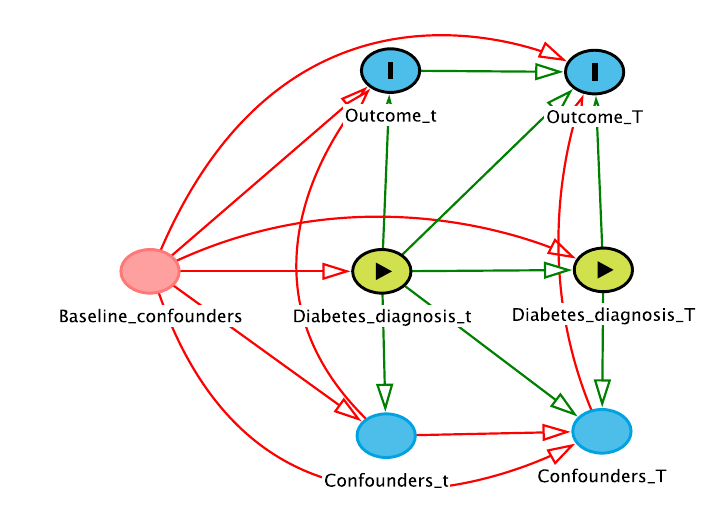
\includegraphics[scale=0.5]{Chapter5/Figures/dag_II_alt}
 \end{center}
\footnotesize{\caption{\label{fig:DAG} Direct acyclic graph (DAG) representing the relations between confounders, a diabetes diagnosis and our six outcomes. Exposure: Diabetes diagnosis.
Outcome: Either BMI, waist circumference, daily calorie consumption, any alcohol consumption, smoking status or employment status. Baseline\_confounders (confounders measured in first year of survey participation either in 1997, 2000, 2004, 2006 or 2009): age, age squared, education, province, urbanization index, marital status, han ethnicity, health inurance, living in a rural area, employment status, BMI, waist circumference, daily calorie consumption, any alcohol consumption and smoking status.
Confounders\_t (confounding measured in waves following the baseline wave): age, age squared, education, province, urbanization index, marital status, han ethnicity, health inurance, living in a rural area, employment status, BMI, waist circumference, daily calorie consumption, any alcohol consumption and smoking status. Confounders\_T are confounders measured in the last year of survey participation and are the same as in counfounders\_t. The green paths represent causal relationships; the red paths represent biased relationships.}}
\end{figure}

REDO FIGURE USING WAVE\_T, WAVE\_t+1. WAVE\_t+2, WAVE\_T AS IN Using Marginal Structural Modeling to Estimate the Cumulative Impact of an Unconditional Tax Credit on Self-Rated Health
We use two statistical approaches to account for potential confounding. First we use \acp{MSM}, which apply inverse probability weights to adjust for confounding and selection bias as a result of time-varying confounders being affected by prior exposure \autocite{Robins2000}. Under the assumption of the \ac{MSM}\autocite{Robins2000} ---consistency, no unmeasured confounders (exchangability) and positivity (see Discussion section for a discussion of the validity of these assumptions in our case)--- the causal DAG shown in Figure \ref{fig:DAG} displays the association between confounders, exposure and outcome.\footnote{This causal graph was drawn using DAGitty program version 2.3.\autocite{Textor2011}}. 

We account for two sets of confounders: time-invariant variables and time-varying variables at baseline as well as time-varying variables in the waves following the baseline, to capture the effects of changes in these variables over time. In our context it seems possible that, e.g. \ac{BMI} affects the probability of being diagnosed with diabetes which then itself may affect subsequent \ac{BMI} levels, confounding the relationship between a diabetes diagnosis and \ac{BMI} due to selection effects. Similarly for employment, employment history and current employment may affect the probability of self-reporting a diabetes diagnosis through the effect on lifestyle via, e.g. an increase in disposable income or a reduction in leisure time, potentially confounding the relationship between a diabetes diagnosis and employment status. 

Using \ac{MSM} and creating inverse probability of treatment weights we are able to construct a pseudo population, based on the person's potential exposure at each time point, that allows us to adjust the estimates for confounding. We create weights separately for the overall sample, where we include a gender indicator as an additional confounder, and also for males and females. The weights are constructed based on the probability of an individual having the observed exposure given their covariates using the the methods described in \textcite{Cole2008}\autocite{Cole2008}. We first construct unstabilized weights using baseline values of the time-invariant and time-variant confounders as well as time-variant confounders measured at all waves prior to treatment. Because unstabilized weights can be highly variable it is recommended to stabilize the weights estimating treatment probabilities using only time-invariant confounders and baseline information of the time-variant confounders. The stabilized weights range from 0.28 to 15.16 with a mean of 1.00 for the overall sample, and are even narrower for the samples stratified by gender (Table \ref{tab:stabweights}). To further limit the influence of the most extreme weights we also create truncated weights using the 1st and 99th percentile as cut off points.

While \acp{MSM} for pre-treatment selection on observable and time-varying confounders, it assumes that there are no time-invariant unobserved confounders such as family background, cognitive abilities, motivation and other personal characteristics. This is a strong assumption that may be violated. We therefore use linear and logistic fixed effects models for continuous and binary outcomes, respectively,  with estimators that rely only on the within-person variation for identification, thereby accounting for any time-invariant confounding.

The \acp{MSM} are estimated using \ac{OLS} for the continuous outcomes and a logit model for the binary outcomes, weighting all models by the stabilized weights constructed beforehand while adjusting for baseline and time.invariant covariates. Heteroscesticity robust standard errors are used throughout. The results for the binary outcomes of employment status, alcohol consumption and smoking are presented in odds ratios, while the results for \ac{BMI}, waist circumference and calorie consumption are standard beta coefficients. In our primary analysis, we present the results of the \ac{MSM} with untruncated stabilized weights, given that these present unbiased estimates if the assumptions underlying the \ac{MSM} are true. In our sensitivity analysis we use weights truncated at the 1st and 99th percentile to reduce the influence of the most extreme weights.

To deal with missing data, we use chained multiple imputation to impute the missing values. We do not impute missing diabetes information and instead assume that once a diabetes diagnosis was reported, the individual had diabetes in every ensuing wave, even when the observation was missing. If no diabetes was reported in any wave, we assumed that the individual never had diabetes. Consequently, we only imputed missing values for those observations that had a non-missing diabetes status. \footnote{Imputation was carried out in Stata 13.1 with the user-written ICE command.}

\section*{Results}

From the descriptive statistics, we can observe that people with self-reported diabetes are less likely to be employed. Looking at health behaviours, it is mainly men that smoke and drink and very few women report smoking or drinking alcohol. The prevalence of smoking and drinking is lower for men with diabetes and they also consume fewer calories. Further, the self-reported diabetes group has both higher \ac{BMI} and waist circumference levels. They are also older, live in more urbanized areas, are more likely to have insurance and men are somewhat better educated while women are less educated compared to their counterparts. Both men and women report an average time since diagnosis of around 6 years.



\begin{table}[h]
\caption{\label{tab:descriptives_diab}Sample means for males and females, by diabetes status}
\begin{center}
\begin{adjustbox}{max width=\linewidth}  
{
\def\sym#1{\ifmmode^{#1}\else\(^{#1}\)\fi}
\begin{tabular}{l*{4}{c}}
\toprule
                    &\multicolumn{2}{c}{No Diabetes}&\multicolumn{2}{c}{Diabetes}\\\cmidrule(lr){2-3}\cmidrule(lr){4-5}
                    &\multicolumn{1}{c}{Males}&\multicolumn{1}{c}{Females}&\multicolumn{1}{c}{Males}&\multicolumn{1}{c}{Females}\\
\midrule
Employed            &        0.79&        0.64&        0.58&        0.28\\
Smokes              &        0.58&        0.03&        0.46&        0.03\\
Any alcohol consumption&        0.63&        0.10&        0.53&        0.07\\
Kcal (3-day average)&     2403.72&     2033.78&     2203.09&     2001.40\\
\ac{BMI}                 &       23.06&       23.14&       24.89&       25.37\\
Waist circ. (cm)    &       82.35&       78.82&       88.91&       86.57\\
Age                 &       42.90&       43.16&       53.06&       54.85\\
Han ethnicity       &        0.88&        0.88&        0.91&        0.93\\
Rural area          &        0.66&        0.66&        0.49&        0.45\\
Married             &        0.82&        0.85&        0.95&        0.86\\
Secondary educ.     &        0.64&        0.50&        0.63&        0.45\\
University educ.    &        0.07&        0.06&        0.15&        0.03\\
Any health insurance&        0.53&        0.52&        0.74&        0.65\\
Urbanization Index  &       62.54&       63.21&       76.13&       71.09\\
Years since diabetes diagnosis&        -&        -&        6.21&        6.34\\
\midrule
Observations        &       25137&       27042&         436&         444\\
\bottomrule
\end{tabular}
}
\end{adjustbox}
\end{center}
\end{table}
\FloatBarrier

The results of our regression analysis are presented in Table \ref{tab:binary}. Both the \ac{FE} model and the \ac{MSM} indicate that women self-reporting a diabetes diagnosis have lower odds of being employed than their counterparts without diabetes, with the \ac{FE} model indicating a larger reduction (0.307 [.154,.613]) compared to the \ac{MSM} (0.583 [.457,.744]). For men no such effect is observed. %reduction of at least 8 p.p. (MSM) for women.

\begin{table}[h]

\caption{\label{tab:binary}Analysis of the effect of a diabetes diagnosis on employment status and behavioral outcomes using fixed effects and marginal structural models}
\begin{adjustbox}{max width=\textwidth, center}
\begin{threeparttable}  %adds notes to tables
{
\def\sym#1{\ifmmode^{#1}\else\(^{#1}\)\fi}
\begin{tabular}{l*{6}{D{.}{.}{-1}l}} \toprule
                &\multicolumn{3}{c}{Odds ratios}                   &\multicolumn{3}{c}{Beta coefficients}             \\\cmidrule(lr){2-4}\cmidrule(lr){5-7}
                &\multicolumn{1}{c}{(1)}&\multicolumn{1}{c}{(2)}&\multicolumn{1}{c}{(3)}&\multicolumn{1}{c}{(4)}&\multicolumn{1}{c}{(5)}&\multicolumn{1}{c}{(6)}\\
                &\multicolumn{1}{c}{Employment}&\multicolumn{1}{c}{Smoking}&\multicolumn{1}{c}{Any alcohol}&\multicolumn{1}{c}{\ac{BMI}}&\multicolumn{1}{c}{Waist (cm)}&\multicolumn{1}{c}{Calories (kcal)}\\
&\multicolumn{6}{c}{\emph{Fixed effects}} \\  
\addlinespace                                   
Complete sample &&&&&&\\                
Diabetes         &            .683&            .776&            .532&           -.658&          -1.408&        -104.058\\
                &    [.449,1.037]&    [.475,1.267]&     [.348,.814]&   [-.910,-.407]&  [-2.213,-.602]&[-194.055,-14.061]\\
\midrule
Male sample &&&&&&\\
Diabetes        &           1.378&            .948&            .568&           -.733&          -1.983&        -164.450\\
                &    [.780,2.437]&    [.566,1.587]&     [.351,.918]&  [-1.111,-.355]&  [-3.164,-.802]&[-307.400,-21.499]\\
\midrule
Female sample &&&&&&\\
Diabetes      &            .307&            .075&            .452&           -.633&           -.951&         -46.637\\
                &     [.154,.613]&     [.008,.691]&    [.178,1.145]&   [-.972,-.295]&   [-2.060,.158]&[-159.060,65.785]\\          
\addlinespace 
&\multicolumn{6}{c}{\emph{Marginal structural model}} \\
\addlinespace             
Complete sample &&&&&&\\                
Diabetes        &       .553&            .881&            .590&            .290&           -.469&         -55.868\\
                &   [.464,.660]&    [.658,1.179]&     [.470,.740]&    [-.415,.995]&   [-1.126,.188]&[-108.440,-3.297]\\
\midrule
Male sample &&&&&&\\
Diabetes        &         .791&            .867&            .583&                -.255&           -.841&         -65.562\\
                &    [.588,1.063]&    [.635,1.182]&     [.444,.766]&   [-.570,.060]&   [-1.902,.220]&[-165.751,34.628]\\
\midrule
Female sample &&&&&&\\
Diabetes        &           .583&            .524&            .565&            .598&           -.217&         -39.216\\
                &   [.457,.744]&    [.252,1.092]&     [.371,.861]&    [-.292,1.488]&   [-1.190,.756]&[-94.555,16.122]\\                
\bottomrule
\end{tabular}
\begin{tablenotes}
\item Notes: 95\% confidence intervals in brackets. Other control variables: age squared, region, urban, education, han, marital status, urbanicity index, time dummies, health insurance status.  N=48934 (pooled sample), N=24321 (male sample), N=24613 (female sample).
\end{tablenotes}
}
\end{threeparttable}
\end{adjustbox}

\end{table}

There is a more ambiguous picture for the effect of a diabetes diagnosis on behavioral outcomes. It does not appear that men reduce their smoking rate, however, there is evidence that a diabetes diagnosis decreases alcohol consumption supported by both models. For waist circumference, \ac{BMI} and calorie consumption, the \ac{FE} models suggests a reduction of -.733 [-1.111,-.355] for \ac{BMI}, about -1.98 [-3.164,-.802] cm in waist circumference and -164.450 [-307.400,-21.499] calories per day. However, the \acp{MSM} do not find similar strong effects and confidence intervals include the null throughout.

Exploring the effect of a diabetes diagnosis over time, we first estimate a specification using time since diagnosis as a continuous variable. The results of the \ac{FE} model (Table \ref{tab:duration}), indicate a steady reduction of female employment odds (.924 [.854,1.000]) and of male \ac{BMI}  (-.096 [-.152,-.039]) and waist circumference (-.347 [-.524,-.170]). Here, the \ac{MSM} supports the finding of a reduction in \ac{BMI} (.032 [-.060,-.005]) and waist circumference (-.133 [-.233,-.032]), albeit with effect sizes only about one-third as large. It also indicates a yearly reduction in calorie consumption. The reduction in employment odds is similar to that found by the \ac{FE} model. 

\begin{table}[h]
\caption{\label{tab:duration}Analysis of the effect of time since diabetes diagnosis on employment status and behavioral outcomes using fixed effects and marginal structural models}
\begin{adjustbox}{max width=\linewidth} 
\begin{threeparttable}  %adds notes to tables
{
\def\sym#1{\ifmmode^{#1}\else\(^{#1}\)\fi}
\begin{tabular}{l*{6}{D{.}{.}{-1}l}} \toprule
                &\multicolumn{3}{c}{Odds ratios}                   &\multicolumn{3}{c}{Beta coefficients}         \\\cmidrule(lr){2-4}\cmidrule(lr){5-7}
                &\multicolumn{1}{c}{(1)}&\multicolumn{1}{c}{(2)}&\multicolumn{1}{c}{(3)}&\multicolumn{1}{c}{(4)}&\multicolumn{1}{c}{(5)}&\multicolumn{1}{c}{(6)}\\
                &\multicolumn{1}{c}{Employment}&\multicolumn{1}{c}{Smoking}&\multicolumn{1}{c}{Any alcohol}&\multicolumn{1}{c}{\ac{BMI}}&\multicolumn{1}{c}{Waist (cm)}&\multicolumn{1}{c}{Calories (kcal)}\\
                \midrule
&\multicolumn{6}{c}{\emph{Fixed effects}} \\
\addlinespace                     
Complete sample &&&&&&\\                
Time since diagnosis&            .983&            .996&            .937&           -.066&           -.234&         -12.742\\
                &    [.927,1.044]&    [.924,1.074]&     [.881,.996]&   [-.104,-.028]&   [-.358,-.110]& [-28.028,2.544]\\
\midrule
Male sample &&&&&&\\
Time since diagnosis&           1.057&           1.014&            .929&           -.096&           -.347&         -17.599\\
                &    [.975,1.147]&    [.938,1.097]&    [.861,1.002]&   [-.152,-.039]&   [-.524,-.170]& [-39.723,4.524]\\
\midrule
Female sample &&&&&&\\
Time since diagnosis&            .924&            .860&            .959&           -.045&           -.155&          -9.136\\
                &    [.854,1.000]&    [.685,1.081]&    [.866,1.061]&    [-.097,.007]&    [-.327,.017]&[-30.556,12.284]\\ 
\addlinespace 
&\multicolumn{6}{c}{\emph{Marginal structural model}} \\               
\addlinespace 
Complete sample &&&&&&\\                
Time since diagnosis   &.957&            .979&            .946&          -.001&           -.070&          -5.800\\
                &   [.937,.977]&    [.943,1.017]&     [.921,.972]&    [-.029,.027]&   [-.139,-.001]& [-11.006,-.595]\\
\midrule
Male sample &&&&&&\\
Time since diagnosis     &.974&            .981&            .940&         -.032&           -.133&          -9.777\\
                &    [.944,1.006]&    [.943,1.020]&     [.911,.969]&    [-.060,-.005]&   [-.233,-.032]&[-18.434,-1.119]\\
\midrule
Female sample &&&&&&\\
Time since diagnosis        &.953&            .919&            .960&            .028&           -.042&          -2.846\\
                &[.930,.976]&    [.835,1.012]&    [.918,1.004]&    [-.015,.070]&    [-.142,.059]&  [-8.918,3.225]\\                 
\bottomrule
\end{tabular}
\begin{tablenotes}
\item Notes: 95\% confidence intervals in brackets. Other control variables: age squared, region, urban, education, han, marital status, urbanicity index, time dummies, health insurance status. N=48934 (pooled sample), N=24321 (male sample), N=24613 (female sample).
\end{tablenotes}
}
\end{threeparttable}
\end{adjustbox}
\end{table}

\FloatBarrier

In a second step we estimate a specification using year dummies to capture the potential non-linearity in the relationship between time since diagnosis and our outcomes. The results of the \ac{FE} model are presented in Table \ref{tab:duration_groups_fe} and of the \ac{MSM} in Table \ref{tab:duration_groups_msm}. Despite the smaller sample size in each group and hence lower precision, the \ac{FE} model still indicates a reduction in \ac{BMI} and waist circumference for men, especially in the first 8 to 10 years after diagnosis, after which they appear to remain stable. A similar effect is found for females, especially for years 3 to 8 after diagnosis. We do not find a strong immediate effect of the diagnosis as shown by the results for year 0. Interestingly, female employment odds already decrease rapidly in the 1 to 2 year after diagnosis and stabilize thereafter at a very low level. Using the \ac{MSM}, all point estimates suggest similar effects, though the effect sizes are again much smaller and confidence intervals include the one or null for the logit and linear models, repectively, throughout.






\begin{table}[hp]
\caption{\label{tab:duration_groups_fe}Analysis of the effect of time since diabetes diagnosis on employment status and behavioral outcomes using fixed effects (duration groups)}
\begin{adjustbox}{max width=\linewidth} 
\begin{threeparttable} 
{
\def\sym#1{\ifmmode^{#1}\else\(^{#1}\)\fi}
\begin{tabular}{l*{6}{D{.}{.}{-1}l}} \toprule
                &\multicolumn{3}{c}{Odds ratios}                   &\multicolumn{3}{c}{Beta coefficients}         \\\cmidrule(lr){2-4}\cmidrule(lr){5-7}
                &\multicolumn{1}{c}{(1)}&\multicolumn{1}{c}{(2)}&\multicolumn{1}{c}{(3)}&\multicolumn{1}{c}{(4)}&\multicolumn{1}{c}{(5)}&\multicolumn{1}{c}{(6)}\\
                &\multicolumn{1}{c}{Employment}&\multicolumn{1}{c}{Smoking}&\multicolumn{1}{c}{Any alcohol}&\multicolumn{1}{c}{\ac{BMI}}&\multicolumn{1}{c}{Waist (cm)}&\multicolumn{1}{c}{Calories (kcal)}\\
                \midrule            
Complete sample &&&&&&\\                     
0               &           1.421&           1.242&            .895&           -.316&           -.990&        -119.626\\
                &    [.336,6.018]&    [.250,6.175]&    [.260,3.082]&   [-1.120,.489]&  [-3.921,1.941]&[-411.165,171.913]\\

1-2             &            .711&            .701&            .529&           -.526&           -.819&        -156.314\\
                &    [.430,1.175]&    [.367,1.338]&     [.306,.915]&   [-.844,-.209]&   [-1.830,.191]&[-270.452,-42.176]\\

3-4             &            .634&            .933&            .482&           -.662&          -1.472&         -19.514\\
                &    [.347,1.158]&    [.457,1.906]&     [.257,.902]&  [-1.027,-.296]&  [-2.671,-.273]&[-157.794,118.766]\\

5-6             &            .560&            .642&            .546&           -.907&          -2.273&         -81.918\\
                &    [.267,1.174]&    [.262,1.574]&    [.257,1.160]&  [-1.370,-.444]&  [-3.726,-.819]&[-267.932,104.096]\\

7-8             &            .570&            .645&            .423&          -1.216&          -3.475&         -91.257\\
                &    [.225,1.443]&    [.184,2.262]&    [.158,1.127]&  [-1.792,-.641]& [-5.399,-1.551]&[-311.703,129.188]\\

9-10            &            .662&            .748&            .465&          -1.144&          -3.302&        -166.003\\
                &    [.251,1.746]&    [.195,2.874]&    [.142,1.526]&  [-1.871,-.417]& [-5.358,-1.247]&[-419.828,87.821]\\

11-12           &            .926&            .695&            .445&          -1.285&          -3.750&        -218.542\\
                &    [.227,3.780]&    [.131,3.671]&    [.115,1.727]&  [-2.196,-.374]& [-6.396,-1.104]&[-509.075,71.991]\\

13-14           &            .997&            .772&            .398&          -1.131&          -3.772&        -266.263\\
                &    [.282,3.528]&    [.152,3.925]&    [.089,1.783]&  [-2.050,-.212]&  [-6.922,-.622]&[-604.676,72.150]\\

15-19           &            .807&           1.012&            .263&           -.950&          -4.264&        -276.358\\
                &    [.221,2.947]&    [.229,4.474]&     [.072,.955]&  [-1.793,-.107]& [-7.185,-1.344]&[-617.312,64.596]\\

20+             &            .957&           2.661&            .349&          -1.032&          -3.657&        -201.122\\
                &    [.152,6.036]& [.000,6.6e+216]&    [.051,2.387]&   [-2.441,.377]&   [-8.109,.795]&[-689.722,287.478]\\
\midrule
Male sample &&&&&&\\
0               &           3.045&           1.084&            .752&           -.229&           -.130&         -87.682\\
                &   [.134,69.100]&    [.203,5.785]&    [.196,2.880]&   [-1.400,.941]&  [-4.067,3.806]&[-551.388,376.024]\\

1-2             &           1.520&            .893&            .579&           -.707&          -1.357&        -236.906\\
                &    [.755,3.059]&    [.456,1.748]&    [.314,1.067]&  [-1.183,-.231]&   [-2.846,.131]&[-418.413,-55.400]\\

3-4             &           1.155&           1.125&            .516&           -.674&          -2.431&        -115.922\\
                &    [.497,2.683]&    [.526,2.406]&    [.261,1.022]&  [-1.196,-.152]&  [-4.118,-.744]&[-339.297,107.452]\\

5-6             &            .910&            .830&            .596&           -.920&          -2.598&         -34.146\\
                &    [.293,2.827]&    [.307,2.246]&    [.241,1.469]&  [-1.612,-.228]&  [-4.893,-.302]&[-306.902,238.611]\\

7-8             &           1.668&            .593&            .519&          -1.128&          -4.527&        -109.609\\
                &    [.404,6.879]&    [.136,2.590]&    [.161,1.680]&  [-2.031,-.225]& [-7.421,-1.632]&[-456.156,236.937]\\

9-10            &           2.184&            .855&            .409&          -1.541&          -5.643&        -217.116\\
                &    [.508,9.395]&    [.195,3.761]&    [.112,1.501]&  [-2.579,-.503]& [-8.725,-2.561]&[-609.350,175.117]\\

11-12           &           3.034&            .977&            .453&          -1.530&          -5.116&        -318.057\\
                &   [.567,16.229]&    [.163,5.845]&    [.086,2.379]&  [-2.831,-.229]& [-9.014,-1.218]&[-820.996,184.882]\\

13-14           &           3.077&           1.016&            .334&          -1.264&          -5.292&        -414.310\\
                &   [.481,19.668]&    [.174,5.921]&    [.057,1.951]&   [-2.621,.093]&  [-9.692,-.891]&[-911.828,83.209]\\

15-19           &           3.174&           1.339&            .252&          -1.435&          -4.997&        -279.397\\
                &   [.548,18.372]&    [.284,6.312]&    [.052,1.229]&  [-2.606,-.265]&  [-9.200,-.795]&[-733.257,174.464]\\

20+             &           4.363&           3.044&            .372&          -2.005&          -7.307&        -296.654\\
                & [.000,1.7e+198]& [.000,1.2e+176]& [.000,9.29e+71]&   [-4.251,.242]&  [-15.495,.881]&[-1198.750,605.441]\\
\midrule
Female sample &&&&&&\\
0               &            .738&        7986.670&           1.565&           -.440&          -1.792&        -143.450\\
                &    [.118,4.633]&        [.000,.]&   [.103,23.811]&   [-1.577,.697]&  [-5.988,2.404]&[-496.408,209.508]\\

1-2             &            .277&            .004&            .385&           -.394&           -.354&         -80.284\\
                &     [.118,.648]&        [.000,.]&    [.101,1.463]&    [-.814,.025]&  [-1.732,1.024]&[-220.575,60.007]\\

3-4             &            .332&            .105&            .380&           -.694&           -.629&          78.022\\
                &     [.132,.833]&    [.007,1.681]&    [.075,1.935]&  [-1.230,-.159]&  [-2.423,1.166]&[-94.574,250.617]\\

5-6             &            .313&            .005&            .441&           -.953&          -2.170&        -113.113\\
                &     [.112,.875]&        [.000,.]&    [.090,2.160]&  [-1.618,-.287]&  [-4.237,-.104]&[-349.303,123.076]\\

7-8             &            .209&           1.231&            .244&          -1.332&          -2.871&         -66.211\\
                &     [.050,.870]&        [.000,.]&    [.021,2.780]&  [-2.047,-.617]&  [-5.341,-.400]&[-350.276,217.855]\\

9-10            &            .180&           1.670&            .861&           -.853&          -1.469&        -110.170\\
                &     [.038,.856]&        [.000,.]&    [.081,9.128]&   [-1.795,.089]&  [-4.379,1.441]&[-438.641,218.301]\\

11-12           &            .233&                &            .495&          -1.105&          -2.795&        -129.937\\
                &    [.026,2.088]&                &    [.033,7.472]&   [-2.429,.220]&  [-6.627,1.037]&[-486.493,226.618]\\

13-14           &            .267&                &            .682&          -1.060&          -2.469&        -120.575\\
                &    [.038,1.878]&                &   [.038,12.372]&   [-2.446,.325]&  [-6.489,1.551]&[-547.082,305.933]\\

15-19           &            .187&                &            .339&           -.535&          -3.712&        -266.417\\
                &    [.029,1.188]&                &    [.025,4.587]&   [-1.771,.700]&   [-7.666,.243]&[-763.937,231.103]\\

20+             &            .211&                &            .497&           -.426&          -1.602&        -147.136\\
                &    [.020,2.195]&                &    [.031,8.023]&  [-2.404,1.553]&  [-7.368,4.163]&[-806.223,511.951]\\              
\bottomrule
\end{tabular}
\begin{tablenotes}
\item Notes: Coefficients for employment, smoking and alcohol models represent odds ratios;  95\% confidence intervals in brackets.
Other control variables: age squared, region, urban, education, han, marital status, urbanicity index, time dummies, health insurance status. N=48934 (pooled sample), N=24321 (male sample), N=24613 (female sample).

\end{tablenotes}
}
\end{threeparttable}
\end{adjustbox}
\end{table}


\begin{table}[hp]
\caption{\label{tab:duration_groups_msm}Analysis of the effect of time since diabetes diagnosis on employment status and behavioral outcomes using marginal structural models (duration groups)}
\begin{adjustbox}{max width=\linewidth}  
\begin{threeparttable}
{
\def\sym#1{\ifmmode^{#1}\else\(^{#1}\)\fi}
\begin{tabular}{l*{6}{D{.}{.}{-1}l}} \toprule
                &\multicolumn{3}{c}{Odds ratios}                   &\multicolumn{3}{c}{Beta coefficients}         \\\cmidrule(lr){2-4}\cmidrule(lr){5-7}
                &\multicolumn{1}{c}{(1)}&\multicolumn{1}{c}{(2)}&\multicolumn{1}{c}{(3)}&\multicolumn{1}{c}{(4)}&\multicolumn{1}{c}{(5)}&\multicolumn{1}{c}{(6)}\\
                &\multicolumn{1}{c}{Employment}&\multicolumn{1}{c}{Smoking}&\multicolumn{1}{c}{Any alcohol}&\multicolumn{1}{c}{\ac{BMI}}&\multicolumn{1}{c}{Waist (cm)}&\multicolumn{1}{c}{Calories (kcal)}\\
                \midrule            
Complete sample &&&&&&\\                
0               &           1.324&           2.174&            .937&            .471&           2.448&         -38.611\\
                &    [.564,3.107]&    [.797,5.933]&    [.342,2.566]&   [-.506,1.448]&  [-1.123,6.020]&[-257.248,180.026]\\

1-2             &            .819&           1.033&            .769&           1.687&           -.234&         -68.721\\
                &    [.609,1.102]&    [.633,1.687]&    [.503,1.175]&   [-.876,4.250]&   [-1.457,.989]&[-170.991,33.549]\\

3-4             &            .704&            .919&            .560&           -.154&            .158&           1.896\\
                &    [.487,1.018]&    [.521,1.621]&     [.341,.920]&    [-.537,.230]&  [-1.105,1.420]&[-173.148,176.939]\\

5-6             &            .549&            .736&            .567&           -.316&           -.339&         -66.028\\
                &     [.351,.860]&    [.330,1.642]&     [.327,.985]&    [-.709,.077]&  [-1.677,1.000]&[-224.072,92.016]\\

7-8             &            .649&            .751&            .563&           -.544&          -1.371&         -18.005\\
                &    [.379,1.113]&    [.323,1.748]&    [.277,1.143]&   [-.994,-.095]&   [-2.921,.178]&[-175.759,139.749]\\

9-10            &            .498&            .732&            .544&           -.418&          -1.034&         -75.109\\
                &     [.272,.911]&    [.266,2.016]&    [.230,1.288]&    [-.984,.149]&   [-2.819,.751]&[-231.855,81.637]\\

11-12           &            .459&            .852&            .499&           -.181&          -1.416&         -98.551\\
                &    [.210,1.002]&    [.207,3.496]&    [.180,1.387]&    [-.919,.557]&   [-3.521,.689]&[-300.671,103.570]\\

13-14           &            .559&            .697&            .456&           -.092&           -.845&        -115.108\\
                &    [.255,1.226]&    [.194,2.498]&    [.164,1.270]&    [-.892,.707]&  [-3.420,1.730]&[-346.553,116.338]\\

15-19           &            .600&            .800&            .400&            .278&          -1.385&        -106.993\\
                &    [.314,1.143]&    [.230,2.782]&    [.156,1.030]&   [-.711,1.268]&   [-3.423,.654]&[-270.748,56.761]\\

20+             &            .566&            .549&            .554&            .195&           -.390&         -26.409\\
                &    [.202,1.589]&    [.058,5.223]&    [.129,2.376]&   [-.964,1.354]&  [-4.376,3.595]&[-319.359,266.541]\\
\midrule
Male sample &&&&&&\\
0               &           1.964&           1.792&           1.021&            .788&           4.180&          12.529\\
                &    [.415,9.285]&    [.569,5.646]&    [.266,3.914]&  [-1.226,2.802]& [-2.662,11.021]&[-335.805,360.862]\\

1-2             &            .888&           1.008&            .818&           -.032&            .270&         -19.756\\
                &    [.491,1.606]&    [.609,1.668]&    [.481,1.391]&    [-.700,.637]&  [-1.558,2.099]&[-284.611,245.098]\\

3-4             &            .861&            .930&            .657&           -.314&           -.793&         -45.068\\
                &    [.410,1.808]&    [.531,1.628]&    [.371,1.163]&    [-.883,.254]&  [-2.658,1.072]&[-329.138,239.001]\\

5-6             &            .584&            .751&            .532&           -.360&           -.729&           5.726\\
                &    [.291,1.170]&    [.344,1.643]&    [.276,1.024]&    [-.916,.197]&  [-2.907,1.448]&[-214.882,226.334]\\

7-8             &            .789&            .597&            .614&           -.448&          -2.090&         -26.423\\
                &    [.344,1.808]&    [.248,1.436]&    [.269,1.399]&   [-1.064,.167]&   [-4.596,.415]&[-293.398,240.553]\\

9-10            &            .680&            .796&            .499&           -.532&          -2.394&        -131.115\\
                &    [.251,1.848]&    [.277,2.287]&    [.187,1.335]&   [-1.364,.301]&   [-5.148,.359]&[-409.533,147.303]\\

11-12           &            .653&            .937&            .457&           -.488&          -2.092&        -161.466\\
                &    [.181,2.359]&    [.215,4.077]&    [.138,1.507]&   [-1.387,.412]&  [-5.336,1.151]&[-529.177,206.246]\\

13-14           &            .751&            .749&            .425&           -.198&          -1.750&        -223.623\\
                &    [.234,2.407]&    [.192,2.920]&    [.142,1.269]&   [-1.094,.697]&  [-4.975,1.475]&[-580.549,133.302]\\

15-19           &            .850&            .849&            .348&           -.420&          -1.792&        -139.844\\
                &    [.303,2.384]&    [.234,3.076]&     [.125,.967]&   [-1.263,.423]&  [-4.988,1.405]&[-420.088,140.400]\\

20+             &            .764&            .587&            .343&           -.523&          -1.926&        -223.129\\
                &    [.084,6.953]&    [.049,6.992]&    [.044,2.710]&  [-2.344,1.299]&  [-8.615,4.763]&[-844.647,398.390]\\
\midrule
Female sample &&&&&&\\
0               &           1.412&           3.253&            .785&            .548&           1.962&        -122.785\\
                &    [.365,5.460]&   [.379,27.904]&    [.078,7.948]&   [-.779,1.875]&  [-3.972,7.895]&[-404.285,158.715]\\

1-2             &            .635&            .657&            .640&           2.315&           -.338&         -48.781\\
                &    [.397,1.016]&    [.219,1.966]&    [.218,1.882]&   [-.955,5.584]&  [-2.139,1.463]&[-158.737,61.174]\\

3-4             &            .579&            .584&            .312&           -.031&            .968&           5.306\\
                &    [.321,1.044]&    [.060,5.713]&    [.060,1.614]&    [-.535,.472]&  [-1.112,3.048]&[-151.576,162.189]\\

5-6             &            .530&            .214&            .636&           -.230&           -.312&         -75.651\\
                &    [.261,1.079]&    [.017,2.711]&    [.212,1.907]&    [-.757,.297]&  [-1.998,1.374]&[-275.992,124.690]\\

7-8             &            .564&            .873&            .249&           -.656&          -1.092&         -20.452\\
                &    [.269,1.186]&    [.109,6.956]&    [.022,2.790]&   [-1.371,.059]&   [-2.951,.767]&[-225.136,184.231]\\

9-10            &            .416&            .350&            .530&           -.211&           -.015&          -9.277\\
                &    [.157,1.101]&   [.011,11.041]&    [.092,3.073]&   [-1.225,.802]&  [-2.646,2.615]&[-226.488,207.935]\\

11-12           &            .621&                &            .563&            .337&           -.792&         -65.396\\
                &    [.176,2.192]&                &    [.090,3.504]&  [-1.229,1.904]&  [-4.050,2.466]&[-321.362,190.569]\\

13-14           &            .680&                &            .597&            .093&           -.478&         -11.959\\
                &    [.206,2.242]&                &    [.065,5.473]&  [-1.788,1.973]&  [-4.393,3.436]&[-309.621,285.704]\\

15-19           &            .548&                &            .460&           1.081&          -1.567&         -92.951\\
                &    [.230,1.304]&                &    [.054,3.944]&   [-.926,3.088]&  [-4.725,1.590]&[-303.513,117.611]\\

20+             &            .450&                &           1.009&            .604&            .025&          51.625\\
                &    [.152,1.329]&                &    [.269,3.785]&  [-1.500,2.708]&  [-5.110,5.160]&[-260.759,364.008]\\           
\bottomrule
\end{tabular}
\begin{tablenotes}
\item Notes: Coefficients for employment, smoking and alcohol models represent odds ratios;  95\% confidence intervals in brackets. Other control variables: age squared, region, urban, education, han, marital status, urbanicity index, time dummies, health insurance status. N=48934 (pooled sample), N=24321 (male sample), N=24613 (female sample).
\end{tablenotes}
}
\end{threeparttable}
\end{adjustbox}
\end{table}

We conduct three sensitivity analyses. First, we truncate weights at the 1\textsuperscript{st} and 99\textsuperscript{th} percentile to investigate the sensitivity of the \acp{MSM} to the most extreme weights. Effect sizes increase in magnitude and are closer to those of the \ac{FE} models, now more clearly supporting the finding of a reduction in \ac{BMI}, waist circumference and alcohol consumption for men (Table \ref{tab:truncation}). For the binary diagnosis indicator they further suggest a reduction in male smoking (for females as well). Second, we estimate all models using only covariate adjustment to investigate in how far this 'naive' approach diverts from the "causal" estimates of the \ac{FE} and \acp{MSM}. The results show that the bias is particularly strong for \ac{BMI} and waist circumference, where naive regression indicates a positive association with a diabetes diagnosis (Table \ref{tab:binary_cov}). For the other outcomes, the results at least point into the same direction as the \ac{FE} and \acp{MSM}, though still differ in the effect size. Third, we estimate the \ac{FE} and \acp{MSM} using the original non-imputed data. The results are broadly similar, in particular for the \ac{FE} model, still indicating a reduction in female employment chances and male alcohol consumption, \ac{BMI} and waist circumference. The coefficients of the \ac{MSM} still point into the same direction as those using the imputed data, but the estimated effects are smaller in size and confidence intervals relatively large.


\FloatBarrier


\section*{Disussion}

Our results suggest that receiving a diabetes diagnosis in China leads to a lasting reduction in male \ac{BMI} and waist circumference levels as well as in risk behaviours such as alcohol consumption. For females, our primary results do not find as strong indications for behaviour change. However, we find a reduction in female employment odds, suggesting that many women stop working as a result of the diagnosis.
Medical evidence suggest that sustained reductions in weight and body fat can lead to increasing insulin sensitivity, better blood glucose levels and consequently a reduced risk for diabetes related complications. Given our results, it appears that women in China have not been able to make such changes and reduce their risk, potentially hinting at a greater inability of women to loose weight, either due to biological factors or due to inequalities in the access to healthcare and appropriate treatment in the Chinese healthcare system in the studied period. 

\subsubsection*{Limitations}

While we used two estimation methods to reduce the influence of selection bias due to unobserved confounding, one limitation of the used approaches is their inability to account for all forms of selection simultaneously, so that giving our results a causal interpretation is only possible under restrictive assumptions, namely no unobserved time-variant confounding for the \ac{FE} model and positivity, exchangability and consistency for the \ac{MSM}. The assumption of positivity is likely to hold, given than every person should have at least a small chance of receiving a diabetes diagnosis. This is also supported by the relatively small range of stabilized weights. Exchangability or no unmeasured confounding is not testable and could potentially be violated if not all time-invariant or time-variant confounders are accounted for. Consistency refers to the fact that the reported treatment is actually the treatment that was taken. Here, consistency hinges on the question that if a diabetes diagnosis has been reported the person has actually been diagnosed with diabetes. This is likely only violated in very rare cases of misreporting, given that specificity of diabetes self-report is very high in China.\autocite{Yuan2015} The assumption of consistency is therefore likely to hold in this context. 

The results for time since diagnosis may suffer from some reporting bias given that providing the correct year of diagnosis may become increasingly error prone the longer ago such a diagnosis took place, likely making these results somewhat less reliable compared to the binary diabetes indicator. 


\subsubsection*{Potential mechanisms}

The constant reduction in male \ac{BMI} and waist circumference we have found has also been observed in a cohort of Danish patients \autocite{DeFineOlivarius2015}, where weight increased the years preceding diagnosis, while after diagnosis weight decreased. The exact reasons for this decrease were unknown but attributed to motivation changes as a result of the diagnosis, concluding that time around the diagnosis may represent a window of opportunity to obtain long lasting weight change. Nonetheless, reductions in weight may also be the result of treatment initiation with metformin or other diabetes drugs that have been shown to lead to weight reductions.\autocite{Yang2014} Importantly, the reduction in \ac{BMI} in our sample is accompanied by a reduction in waist circumference which might be the more important marker given that in China diabetes incidence has been especially attributed to a high accumulation of visceral fat and central obesity \autocite{Ma2014}. Reductions in waist circumference therefore may have a particular positive effect on diabetes control and the prevention of comorbidities and can also indicate reductions in fat mass irrespective of changes in \ac{BMI} \autocite{Klein2007}.

For women, however, we do not find similar strong evidence for reductions in \ac{BMI} and waist circumference. The relatively smaller effects found for women could indicate that they are less able to change behaviours to foster weight loss, potentially due to their lower educational attainment, which has been indicated as a factor in preventing better glucose control.\autocite{Luo2015} Lower income levels for females may also negatively affect the ability to receive adequate treatment at and following diagnosis, limiting their ability to change health behaviours.\autocite{Luo2015} In this light it might not be surprising that we find more conclusive evidence of worsening employment probabilities for women than for men. If women are less likely to receive proper treatment, the long term effects of diabetes on their health may be more severe than for men and consequently affect their employment status. So has it been shown that diabetes comorbidities are more prevalent in Chinese women than men, indicating that women bear a larger disease burden.\autocite{Liu2010} 

Compared to the only other study that used population level observational data to investigate the effect of a diabetes diagnosis on health behaviours in the \ac{USA} by \textcite{Slade2012}\autocite{Slade2012}, our results paint a somewhat different picture. While Slade finds a more lasting effect on smoking cessation and alcohol consumption, but not on overweight or obesity, our results indicate lasting effects on male alcohol consumption but not on smoking, and we find evidence for a sustained reduction in male body weight. Nonetheless, one has to keep in mind that we used continuous weight indicators in \ac{BMI} and waist circumference, Slade investigated the effect on the probability of being obese or overweight, making a direct comparison difficult. Importantly, and in concordance with our findings he finds that simple covariate adjustment leads to estimates indicating an increase in obesity and overweight underlining the importance of accounting for unobserved heterogeneity and selection on observables.

\section*{Conclusion}

Our results indicate small changes in male health behaviours after diagnosis, robust to the application of two distinct econometric techniques. This provides some evidence that under the healthcare system of the last decade men were able to achieve positive behaviour changes, potentially lowering the burden of diabetes somewhat. Further, women appear to bear a larger diabetes burden also affecting their economic well-being as evidenced by their reduction in employment chances, Further, and potentially contributing to these adverse economic effects, they are less likely to successfully change their behaviour as a result of the diagnosis. Overall, given the large prevalence of undiagnosed diabetes, our results indicate that an early diagnosis can lead to early behaviour change that may lead to more positive health outcomes for people with diabetes over time. It appears, however, that more emphasis on the availability of access to adequate treatment of women may be needed to reduce their burden of diabetes.

\section*{\label{sec:Appendix}Appendix}

\subsection*{Stabilized weights}

\begin{table}[h]
\caption{\label{tab:stabweights}Summary of stabilized weights}
\begin{adjustbox}{max width=\linewidth}  
{
\def\sym#1{\ifmmode^{#1}\else\(^{#1}\)\fi}
\begin{tabular}{l*{1}{ccc}}
\toprule
                    &        Mean&         Min&         Max\\
\midrule
Untruncated (all)   &    1.000471&    .2769484&    15.15908\\
Untruncated (men)   &    1.001343&    .1740716&   5.780513\\
Untruncated (women) &    1.000773&   .1661002&  8.754402\\
Truncated 1 and 99 percentile (all)&    .9994486&    .9011863&    1.073953\\
Truncated 1 and 99 percentile (men)&    .9997768&    .8906016&    1.107517\\
Truncated 1 and 99 percentile (women)&    .9988097&    .8323757&    1.119154\\
Truncated 5 and 95 percentile (all)&    .9997004&    .9889193&    1.013009\\
Truncated 5 and 95 percentile (men)&    .9996405&    .9856438  & 1.01772\\
Truncated 5 and 95 percentile (women)&    .9992396 &    .980685  & 1.019746\\
\bottomrule
\end{tabular}
}
\end{adjustbox}
\end{table}

\FloatBarrier

\subsection*{Predictors of diabetes to calculate stabilized weights}

\begin{table}[h]
\caption{\label{tab:predictors}Predictors of a diabetes diagnosis}
\begin{adjustbox}{max width=\textwidth, center}
\begin{threeparttable}
{
\begin{tabular}{l*{3}{D{.}{.}{-1}l}} \toprule
                &\multicolumn{2}{c}{(1)}   &\multicolumn{2}{c}{(2)}   &\multicolumn{2}{c}{(3)}   \\
                &\multicolumn{2}{c}{Complete sample}&\multicolumn{2}{c}{Male}  &\multicolumn{2}{c}{Female}\\
\midrule
Age (bl)          &     .967&    [.911,1.027]&     .964&    [.890,1.045]&     .973&    [.886,1.068]\\
Age\_sq (bl)       &    1.001&   [1.000,1.001]&    1.001&   [1.000,1.001]&    1.001&   [1.000,1.002]\\
Urbanization Index (bl)        &     .991&    [.978,1.005]&     .999&    [.980,1.018]&     .984&    [.966,1.003]\\
\ac{BMI} (bl)          &    1.204&   [1.131,1.283]&    1.197&   [1.083,1.324]&    1.208&   [1.111,1.313]\\
Waist circumference (cm) (bl)       &    1.035&   [1.016,1.054]&    1.043&   [1.015,1.072]&    1.026&   [1.000,1.053]\\
3-Day Ave: Energy (kcal) (bl)       &    1.000&   [1.000,1.000]&    1.000&   [1.000,1.000]&    1.000&   [1.000,1.000]\\
Smoking (bl) &    1.143&    [.805,1.622]&    1.039&    [.708,1.523]&    2.552&   [1.084,6.012]\\
Any alcohol (bl)     &    1.247&    [.927,1.677]&    1.343&    [.930,1.939]&    1.071&    [.620,1.852]\\
Secondary educ. (bl)   &     .966&    [.635,1.470]&    1.077&    [.604,1.921]&     .875&    [.464,1.652]\\
University (bl)   &     .841&    [.360,1.967]&    1.017&    [.373,2.770]&     .612&    [.085,4.408]\\
Married (bl)     &     .947&    [.580,1.547]&     .919&    [.451,1.871]&    1.046&    [.527,2.077]\\
Any medical insurance (bl)    &    1.137&    [.872,1.482]&    1.262&    [.872,1.826]&    1.045&    [.706,1.546]\\
Employed (bl)        &     .895&    [.676,1.186]&     .630&     [.413,.963]&    1.227&    [.837,1.798]\\
Survey year&&&&&&\\
\hspace*{10mm}2000&     .534&     [.380,.752]&     .343&     [.198,.595]&     .719&    [.459,1.127]\\
\hspace*{10mm}2004&     .498&     [.339,.732]&     .481&     [.279,.830]&     .508&     [.293,.882]\\
\hspace*{10mm}2006&     .457&     [.302,.691]&     .457&     [.257,.813]&     .446&     [.244,.814]\\
\hspace*{10mm}2009&     .903&    [.593,1.377]&    1.026&    [.577,1.823]&     .696&    [.369,1.315]\\
\hspace*{10mm}2011&     .639&    [.391,1.043]&     .493&     [.247,.987]&     .783&    [.386,1.586]\\
Han nationality&     .985&    [.675,1.438]&     .930&    [.555,1.559]&    1.030&    [.588,1.806]\\
Rural           &     .717&     [.570,.902]&     .892&    [.646,1.232]&     .564&     [.406,.785]\\
Female          &     .787&    [.589,1.053]&    1.000&           [.,.]&    1.000&           [.,.]\\
Age&    1.115&   [1.016,1.223]&    1.169&   [1.023,1.337]&    1.037&    [.908,1.184]\\
Age sqared          &     .999&    [.998,1.000]&     .999&    [.997,1.000]&    1.000&    [.998,1.001]\\
\ac{BMI}             &     .906&     [.854,.961]&     .882&     [.803,.968]&     .931&    [.861,1.007]\\
Urbanization Index&    1.004&    [.991,1.017]&    1.006&    [.987,1.025]&    1.001&    [.983,1.020]\\
Waist circumference (cm)&    1.002&    [.984,1.019]&     .998&    [.973,1.024]&    1.001&    [.978,1.025]\\
3-Day Ave: Energy (kcal)&    1.000&   [1.000,1.000]&    1.000&   [1.000,1.000]&    1.000&   [1.000,1.000]\\
Smoking&     .676&     [.475,.963]&     .704&    [.482,1.030]&     .357&    [.122,1.038]\\
Any alcohol&     .596&     [.444,.800]&     .580&     [.412,.815]&     .589&    [.313,1.109]\\
Secondary educ.       &    1.429&    [.936,2.180]&    1.399&    [.775,2.527]&    1.565&    [.836,2.931]\\
University      &    2.144&   [1.010,4.548]&    2.016&    [.805,5.045]&    1.715&    [.356,8.266]\\
Married         &     .948&    [.597,1.504]&    1.227&    [.594,2.534]&     .801&    [.433,1.483]\\
Employed           &     .675&     [.520,.878]&     .960&    [.653,1.413]&     .455&     [.314,.660]\\
Any medical insurance&     .838&    [.631,1.111]&     .739&    [.500,1.092]&    1.008&    [.664,1.529]\\
Employed           &     .675&     [.520,.878]&     .960&    [.653,1.413]&     .455&     [.314,.660]\\
Province&&&&&&\\
\hspace*{10mm}Liaoning        &    1.160&    [.726,1.855]&    1.633&    [.819,3.257]&     .826&    [.427,1.598]\\
\hspace*{10mm}Heilongjiang    &    1.146&    [.723,1.816]&    1.808&    [.923,3.542]&     .652&    [.333,1.279]\\
\hspace*{10mm}Jiangsu         &    1.081&    [.684,1.710]&    1.465&    [.741,2.897]&     .801&    [.426,1.505]\\
\hspace*{10mm}Shandong        &    1.544&   [1.004,2.374]&    2.214&   [1.161,4.224]&    1.084&    [.601,1.955]\\
\hspace*{10mm}Henan           &     .946&    [.598,1.496]&    1.004&    [.487,2.070]&     .854&    [.470,1.553]\\
\hspace*{10mm}Hubei           &    1.099&    [.685,1.763]&    1.374&    [.668,2.824]&     .918&    [.489,1.721]\\
\hspace*{10mm}Hunan           &    1.700&   [1.111,2.602]&    1.984&   [1.036,3.801]&    1.432&    [.809,2.532]\\
\hspace*{10mm}Guizhou         &    1.011&    [.602,1.701]&    1.653&    [.787,3.469]&     .622&    [.294,1.317]\\
\bottomrule
\end{tabular}
\begin{tablenotes}
\item Notes: Exponentiated coefficients; 95\% confidence intervals in brackets.
\end{tablenotes}
}
\end{threeparttable}
\end{adjustbox}
\end{table}


\FloatBarrier

\subsection*{Robusteness checks}
\subsubsection*{Results using non-imputed data}

\begin{table}[h]
\caption{\label{tab:binary_non_mi}Analysis of the effect of a diabetes diagnosis on employment status and behavioral outcomes using fixed effects and marginal structural models (no imputation)}
\begin{adjustbox}{max width=\textwidth, center}
\begin{threeparttable}
{
\def\sym#1{\ifmmode^{#1}\else\(^{#1}\)\fi}
\begin{tabular}{l*{6}{D{.}{.}{-1}l}} \toprule
                &\multicolumn{3}{c}{Odds ratios}                   &\multicolumn{3}{c}{Beta coefficients}             \\\cmidrule(lr){2-4}\cmidrule(lr){5-7}
                &\multicolumn{1}{c}{(1)}&\multicolumn{1}{c}{(2)}&\multicolumn{1}{c}{(3)}&\multicolumn{1}{c}{(4)}&\multicolumn{1}{c}{(5)}&\multicolumn{1}{c}{(6)}\\
                &\multicolumn{1}{c}{Employment}&\multicolumn{1}{c}{Smoking}&\multicolumn{1}{c}{Any alcohol}&\multicolumn{1}{c}{\ac{BMI}}&\multicolumn{1}{c}{Waist (cm)}&\multicolumn{1}{c}{Calories (kcal)}\\
&\multicolumn{6}{c}{\emph{Fixed effects}} \\  
\addlinespace                                   
Complete sample &&&&&&\\                
Diabetes&            .612&            .749&            .587&           -.914&          -1.664&         -51.670\\
                &     [.418,.896]&    [.496,1.130]&     [.415,.830]&  [-1.357,-.471]& [-2.273,-1.055]&[-120.652,17.311]\\
\midrule
Male sample &&&&&&\\
Diabetes&           1.024&            .819&            .602&           -.721&          -1.915&         -69.143\\
                &    [.624,1.680]&    [.523,1.283]&     [.404,.897]&   [-.978,-.464]& [-2.769,-1.060]&[-175.510,37.224]\\
\midrule
Female sample &&&&&&\\
Diabetes&            .303&            .415&            .586&           -.591&          -1.465&         -34.194\\
                &     [.157,.582]&    [.142,1.214]&    [.289,1.187]&   [-.840,-.342]&  [-2.330,-.600]&[-123.117,54.729]\\         
\addlinespace 
&\multicolumn{6}{c}{\emph{Marginal structural model}} \\
\addlinespace             
Complete sample &&&&&&\\                
Diabetes&            .654&            .744&            .595&           -.033&           -.717&         -54.836\\
                &     [.536,.798]&    [.500,1.106]&     [.433,.817]&    [-.321,.255]&  [-1.384,-.051]&[-94.265,-15.408]\\
\midrule
Male sample &&&&&&\\
Diabetes&           1.088&           1.308&           1.126&            .001&           -.150&          25.905\\
                &    [.689,1.718]&    [.875,1.954]&    [.774,1.638]&    [-.263,.264]&   [-1.181,.881]&[-62.266,114.076]\\
\midrule
Female sample &&&&&&\\
Diabetes&            .813&            .900&            .717&            .557&           -.458&          12.660\\
                &    [.562,1.176]&    [.391,2.071]&    [.386,1.333]&   [-.495,1.608]&   [-1.588,.673]&[-59.881,85.200]\\                
\bottomrule
\end{tabular}
\begin{tablenotes}
\item Notes: Coefficients for employment, smoking and alcohol models represent odds ratios;  95\% confidence intervals in brackets.
Other control variables: age squared, region, urban, education, han, marital status, urbanicity index, time dummies, health insurance status. N=34651 (pooled sample), N=15270 (male sample), N=18606 (female sample).
\end{tablenotes}
}
\end{threeparttable}
\end{adjustbox}
\end{table}



\begin{table}[h]
\caption{\label{tab:duration_non_mi}Analysis of the effect of time since diabetes diagnosis on employment status and behavioral outcomes using fixed effects and marginal structural models (non-imputed)}
\begin{adjustbox}{max width=\linewidth}  
\begin{threeparttable}
{
\def\sym#1{\ifmmode^{#1}\else\(^{#1}\)\fi}
\begin{tabular}{l*{6}{D{.}{.}{-1}l}} \toprule
                &\multicolumn{3}{c}{Odds ratios}                   &\multicolumn{3}{c}{Beta coefficients}         \\\cmidrule(lr){2-4}\cmidrule(lr){5-7}
                &\multicolumn{1}{c}{(1)}&\multicolumn{1}{c}{(2)}&\multicolumn{1}{c}{(3)}&\multicolumn{1}{c}{(4)}&\multicolumn{1}{c}{(5)}&\multicolumn{1}{c}{(6)}\\
                &\multicolumn{1}{c}{Employment}&\multicolumn{1}{c}{Smoking}&\multicolumn{1}{c}{Any alcohol}&\multicolumn{1}{c}{\ac{BMI}}&\multicolumn{1}{c}{Waist (cm)}&\multicolumn{1}{c}{Calories (kcal)}\\
                \midrule
&\multicolumn{6}{c}{\emph{Fixed effects}} \\
\addlinespace                     
Complete sample &&&&&&\\                
Time since diagnosis&            .917&            .978&            .955&           -.170&           -.372&          -4.479\\
                &     [.855,.984]&    [.910,1.052]&    [.901,1.013]&   [-.258,-.081]&   [-.475,-.269]& [-16.256,7.297]\\
\midrule
Male sample &&&&&&\\
Time since diagnosis&            .981&            .993&            .909&           -.132&           -.427&          -5.896\\
                &    [.893,1.078]&    [.916,1.076]&     [.843,.980]&   [-.179,-.086]&   [-.580,-.274]&[-25.162,13.370]\\
\midrule
Female sample &&&&&&\\
Time since diagnosis&            .846&            .895&           1.041&           -.102&           -.347&          -3.641\\
                &     [.758,.943]&    [.759,1.057]&    [.947,1.145]&   [-.142,-.062]&   [-.487,-.207]&[-18.072,10.791]\\
\addlinespace 
&\multicolumn{6}{c}{\emph{Marginal structural model}} \\               
\addlinespace 
Complete sample &&&&&&\\                
Time since diagnosis&            .958&            .973&            .971&           -.014&           -.051&          -4.131\\
                &     [.930,.987]&    [.913,1.038]&    [.929,1.015]&    [-.045,.018]&    [-.136,.034]&  [-9.555,1.293]\\
\midrule
Male sample &&&&&&\\
Time since diagnosis&           1.052&           1.032&           1.022&           -.002&           -.033&          -4.850\\
                &    [.993,1.114]&    [.990,1.076]&    [.980,1.065]&    [-.026,.022]&    [-.163,.098]& [-16.694,6.993]\\
\midrule
Female sample &&&&&&\\
Time since diagnosis&            .981&           1.050&           1.013&            .033&            .008&          -1.442\\
                &    [.922,1.044]&    [.999,1.104]&    [.953,1.076]&    [-.025,.091]&    [-.067,.082]&[-13.420,10.537]\\                 
\bottomrule
\end{tabular}
\begin{tablenotes}
\item Notes: Coefficients for employment, smoking and alcohol models represent odds ratios;  95\% confidence intervals in brackets.
Other control variables: age squared, region, urban, education, han, marital status, urbanicity index, time dummies, health insurance status. N=34232 (pooled sample), N=15228 (male sample), N=18547 (female sample).
\end{tablenotes}
}
\end{threeparttable}
\end{adjustbox}
\end{table}


\begin{table}[h]
\caption{\label{tab:duration_groups_non_mi}Analysis of the effect of time since diabetes diagnosis on employment status and behavioral outcomes using fixed effects (duration groups) (non-imputed)}
\begin{adjustbox}{max width=\linewidth}  
\begin{threeparttable}
{
\def\sym#1{\ifmmode^{#1}\else\(^{#1}\)\fi}
\begin{tabular}{l*{6}{D{.}{.}{-1}l}} \toprule
                &\multicolumn{3}{c}{Odds ratios}                   &\multicolumn{3}{c}{Beta coefficients}         \\\cmidrule(lr){2-4}\cmidrule(lr){5-7}
                &\multicolumn{1}{c}{(1)}&\multicolumn{1}{c}{(2)}&\multicolumn{1}{c}{(3)}&\multicolumn{1}{c}{(4)}&\multicolumn{1}{c}{(5)}&\multicolumn{1}{c}{(6)}\\
                &\multicolumn{1}{c}{Employment}&\multicolumn{1}{c}{Smoking}&\multicolumn{1}{c}{Any alcohol}&\multicolumn{1}{c}{\ac{BMI}}&\multicolumn{1}{c}{Waist (cm)}&\multicolumn{1}{c}{Calories (kcal)}\\
                \midrule            
Complete sample &&&&&&\\                
0               &           2.524&           1.066&           1.280&           -.859&           -.809&         -99.831\\
                &   [.464,13.734]&    [.222,5.111]&    [.369,4.436]&   [-2.672,.954]&  [-3.278,1.661]&[-383.264,183.602]\\
\addlinespace
1-2             &            .646&            .628&            .596&           -.812&          -1.297&         -98.584\\
                &    [.399,1.046]&    [.366,1.077]&     [.378,.938]&  [-1.391,-.232]&  [-2.085,-.508]&[-188.060,-9.108]\\
\addlinespace
3-4             &            .535&            .814&            .601&           -.924&          -2.285&          -8.223\\
                &     [.290,.988]&    [.421,1.573]&    [.357,1.012]&  [-1.603,-.245]& [-3.250,-1.321]&[-117.968,101.521]\\
\addlinespace
5-6             &            .407&            .949&            .618&          -1.289&          -2.872&         -27.860\\
                &     [.188,.884]&    [.413,2.180]&    [.296,1.289]&  [-2.189,-.388]& [-4.127,-1.616]&[-169.178,113.459]\\
\addlinespace
7-8             &            .465&            .674&            .567&          -1.102&          -4.410&           5.748\\
                &    [.167,1.296]&    [.191,2.375]&    [.236,1.361]&   [-2.309,.105]& [-5.940,-2.879]&[-169.903,181.399]\\
\addlinespace
9-10            &            .346&            .741&            .348&          -2.486&          -3.489&        -124.163\\
                &    [.117,1.024]&    [.172,3.197]&    [.119,1.023]&  [-4.101,-.871]& [-5.336,-1.641]&[-335.968,87.641]\\
\addlinespace
11-12           &            .498&            .792&            .383&          -1.068&          -5.965&        -107.559\\
                &    [.128,1.929]&    [.179,3.507]&    [.099,1.480]&  [-3.843,1.707]& [-8.210,-3.720]&[-363.893,148.774]\\
\addlinespace
13-14           &            .404&            .632&            .711&          -1.595&          -4.816&        -167.489\\
                &    [.077,2.115]&    [.118,3.383]&    [.171,2.954]&   [-4.180,.990]& [-7.239,-2.393]&[-447.132,112.154]\\
\addlinespace
15-19           &            .552&           1.635&            .516&          -2.253&          -5.747&        -224.284\\
                &    [.090,3.401]&    [.281,9.512]&    [.110,2.423]&   [-5.182,.676]& [-8.370,-3.124]&[-525.502,76.933]\\
\addlinespace
20+             &           1.092&           1.030&            .773&           -.485&          -4.668&          72.707\\
                &    [.132,9.010]&   [.100,10.626]&    [.138,4.338]&  [-6.178,5.208]& [-8.105,-1.231]&[-324.000,469.413]\\
\midrule
Male sample &&&&&&\\
0               &          11.505&           1.127&           1.807&           -.229&          -1.533&        -102.931\\
                &  [.348,380.142]&    [.175,7.277]&    [.409,7.981]&   [-1.311,.853]&  [-5.138,2.072]&[-569.389,363.528]\\
\addlinespace
1-2             &           1.108&            .769&            .690&           -.731&          -1.325&        -119.594\\
                &    [.603,2.035]&    [.432,1.370]&    [.415,1.148]&  [-1.063,-.400]&  [-2.430,-.220]&[-255.994,16.806]\\
\addlinespace
3-4             &            .915&           1.083&            .767&           -.642&          -2.521&        -104.413\\
                &    [.415,2.020]&    [.528,2.221]&    [.429,1.371]&  [-1.033,-.250]& [-3.811,-1.231]&[-267.694,58.867]\\
\addlinespace
5-6             &            .467&           1.162&            .716&          -1.111&          -2.784&          99.891\\
                &    [.153,1.421]&    [.445,3.033]&    [.304,1.684]&  [-1.632,-.591]& [-4.536,-1.032]&[-121.420,321.202]\\
\addlinespace
7-8             &           1.293&            .628&            .661&          -1.214&          -5.004&         -86.535\\
                &    [.260,6.423]&    [.144,2.745]&    [.236,1.848]&  [-1.905,-.522]& [-7.272,-2.736]&[-369.817,196.748]\\
\addlinespace
9-10            &           1.422&            .396&            .198&          -1.604&          -5.852&         -65.915\\
                &    [.365,5.541]&    [.078,2.016]&     [.055,.714]&  [-2.391,-.817]& [-8.468,-3.236]&[-393.401,261.572]\\
\addlinespace
11-12           &           1.397&           1.128&            .169&          -2.025&          -6.181&        -192.234\\
                &    [.239,8.181]&    [.222,5.733]&    [.026,1.103]& [-3.004,-1.046]& [-9.418,-2.944]&[-600.584,216.116]\\
\addlinespace
13-14           &            .726&           1.134&            .460&          -1.214&          -3.286&        -122.290\\
                &    [.066,7.993]&    [.189,6.789]&    [.077,2.743]&  [-2.314,-.113]&   [-6.937,.364]&[-586.610,342.030]\\
\addlinespace
15-19           &           1.875&           1.150&            .325&          -1.473&          -3.826&          83.522\\
                &   [.119,29.590]&    [.174,7.586]&    [.041,2.579]&  [-2.765,-.180]&   [-8.125,.473]&[-451.117,618.161]\\
\addlinespace
20+             &            .000&            .644&            .000&          -1.820&          -4.995&         -30.895\\
                &        [.000,.]&   [.033,12.597]&        [.000,.]&   [-3.740,.100]& [-11.389,1.399]&[-851.432,789.641]\\
\midrule
Female sample &&&&&&\\
0               &            .943&        4.19e+11&            .560&           -.107&           -.208&        -101.978\\
                &    [.089,9.998]&        [.000,.]&    [.038,8.221]&   [-1.081,.866]&  [-3.605,3.189]&[-448.331,244.375]\\
\addlinespace
1-2             &            .239&            .182&            .334&           -.471&          -1.256&         -78.078\\
                &     [.095,.599]&    [.029,1.133]&    [.105,1.061]&   [-.795,-.146]&  [-2.379,-.132]&[-194.744,38.589]\\
\addlinespace
3-4             &            .233&            .104&            .175&           -.684&          -2.114&          97.737\\
                &     [.081,.675]&    [.009,1.134]&     [.039,.778]&  [-1.098,-.271]&  [-3.556,-.672]&[-49.093,244.566]\\
\addlinespace
5-6             &            .241&            .260&            .417&          -1.078&          -2.932&        -129.371\\
                &     [.074,.781]&    [.037,1.838]&    [.081,2.162]&  [-1.590,-.567]& [-4.730,-1.133]&[-309.337,50.595]\\
\addlinespace
7-8             &            .116&            .620&            .462&          -1.300&          -4.117&          82.170\\
                &     [.023,.582]&   [.028,13.943]&    [.072,2.967]&  [-1.904,-.695]& [-6.202,-2.031]&[-135.795,300.134]\\
\addlinespace
9-10            &            .019&        1.47e+24&           2.320&          -1.049&          -1.539&        -180.719\\
                &     [.002,.237]&        [.000,.]&   [.320,16.831]&  [-1.793,-.304]&  [-4.147,1.068]&[-453.281,91.844]\\
\addlinespace
11-12           &            .073&            .000&           3.277&          -1.990&          -6.017&         -37.932\\
                &     [.007,.798]&        [.000,.]&   [.212,50.764]& [-2.865,-1.116]& [-9.139,-2.894]&[-359.316,283.452]\\
\addlinespace
13-14           &            .076&            .000&           2.508&          -1.058&          -5.792&        -158.911\\
                &     [.006,.979]&        [.000,.]&   [.157,40.186]&  [-1.994,-.121]& [-9.078,-2.506]&[-500.863,183.041]\\
\addlinespace
15-19           &            .058&        1.32e+18&           1.659&          -1.640&          -6.765&        -380.410\\
                &     [.004,.892]&        [.000,.]&   [.107,25.704]&  [-2.603,-.676]&[-10.149,-3.382]&[-733.543,-27.278]\\
\addlinespace
20+             &            .118&           1.575&           4.257&          -2.017&          -4.951&          68.302\\
                &    [.007,1.967]&        [.000,.]&   [.300,60.330]&  [-3.217,-.817]&  [-9.168,-.734]&[-370.239,506.842]\\        
\bottomrule
\end{tabular}
\begin{tablenotes}
\item Notes: Coefficients for employment, smoking and alcohol models represent odds ratios;  95\% confidence intervals in brackets.
Other control variables: age squared, region, urban, education, han, marital status, urbanicity index, time dummies, health insurance status. N=34232 (pooled sample), N=15228 (male sample), N=18547 (female sample).
\end{tablenotes}
}
\end{threeparttable}
\end{adjustbox}
\end{table}

\begin{table}[h]
\caption{\label{tab:duration_groups_non_mi}Analysis of the effect of time since diabetes diagnosis on employment status and behavioral outcomes using marginal structural models (duration groups) (non-imputed)}
\begin{adjustbox}{max width=\linewidth}  
\begin{threeparttable}
{
\def\sym#1{\ifmmode^{#1}\else\(^{#1}\)\fi}
\begin{tabular}{l*{6}{D{.}{.}{-1}l}} \toprule
                &\multicolumn{3}{c}{Odds ratios}                   &\multicolumn{3}{c}{Beta coefficients}         \\\cmidrule(lr){2-4}\cmidrule(lr){5-7}
                &\multicolumn{1}{c}{(1)}&\multicolumn{1}{c}{(2)}&\multicolumn{1}{c}{(3)}&\multicolumn{1}{c}{(4)}&\multicolumn{1}{c}{(5)}&\multicolumn{1}{c}{(6)}\\
                &\multicolumn{1}{c}{Employment}&\multicolumn{1}{c}{Smoking}&\multicolumn{1}{c}{Any alcohol}&\multicolumn{1}{c}{\ac{BMI}}&\multicolumn{1}{c}{Waist (cm)}&\multicolumn{1}{c}{Calories (kcal)}\\
                \midrule            
Complete sample &&&&&&\\                
0               &           2.062&           4.541&            .592&            .505&           1.674&         105.356\\
                &    [.901,4.721]&  [1.141,18.064]&    [.237,1.479]&   [-.340,1.350]&  [-1.149,4.498]&[-104.835,315.547]\\
\addlinespace
1-2             &            .797&            .970&            .825&            .418&           -.515&         -58.052\\
                &    [.560,1.135]&    [.510,1.842]&    [.492,1.384]&   [-.649,1.486]&   [-1.684,.653]&[-134.158,18.053]\\
\addlinespace
3-4             &            .752&            .748&            .692&           -.288&           -.998&         -29.731\\
                &    [.485,1.168]&    [.402,1.391]&    [.379,1.262]&    [-.717,.141]&   [-2.286,.290]&[-156.746,97.285]\\
\addlinespace
5-6             &            .588&            .897&            .787&           -.342&           -.448&         -56.715\\
                &     [.357,.968]&    [.388,2.071]&    [.414,1.495]&    [-.806,.122]&   [-1.754,.858]&[-182.786,69.356]\\
\addlinespace
7-8             &            .713&            .566&            .769&           -.464&          -2.004&          22.007\\
                &    [.386,1.315]&    [.220,1.458]&    [.278,2.132]&   [-1.064,.136]&  [-3.741,-.267]&[-136.315,180.329]\\
\addlinespace
9-10            &            .490&            .320&            .552&           -.639&           -.266&         -92.698\\
                &     [.241,.996]&     [.123,.829]&    [.188,1.626]&  [-1.189,-.089]&  [-2.558,2.027]&[-216.351,30.956]\\
\addlinespace
11-12           &            .293&            .559&            .513&           -.524&          -1.867&        -128.512\\
                &     [.128,.672]&    [.111,2.825]&    [.107,2.470]&   [-1.300,.251]&   [-4.282,.547]&[-287.425,30.401]\\
\addlinespace
13-14           &            .405&            .259&            .869&            .136&            .629&        -207.398\\
                &    [.156,1.054]&     [.070,.961]&    [.157,4.826]&    [-.597,.870]&  [-2.396,3.655]&[-399.436,-15.361]\\
\addlinespace
15-19           &            .664&            .534&            .477&            .629&           -.002&        -181.788\\
                &    [.341,1.295]&    [.067,4.275]&    [.128,1.785]&   [-.870,2.129]&  [-2.618,2.614]&[-344.771,-18.806]\\
\addlinespace
20+             &            .927&           1.907&            .844&           -.564&           -.525&         145.138\\
                &    [.333,2.584]&   [.169,21.573]&    [.213,3.345]&   [-1.492,.363]&  [-3.712,2.663]&[-107.404,397.681]\\
\midrule
Male sample &&&&&&\\
0               &          17.267&           5.848&            .740&           -.242&            .188&          93.942\\
                &  [3.540,84.208]&  [1.004,34.062]&    [.243,2.249]&   [-1.280,.797]&  [-1.787,2.162]&[-114.186,302.070]\\
\addlinespace
1-2             &           1.017&           1.452&           1.375&            .019&           -.065&         -10.903\\
                &    [.499,2.073]&    [.739,2.853]&    [.692,2.731]&    [-.480,.519]&  [-1.699,1.570]&[-150.313,128.507]\\
\addlinespace
3-4             &           2.291&            .898&           1.323&           -.407&          -1.967&        -201.354\\
                &    [.960,5.468]&    [.364,2.211]&    [.781,2.240]&   [-.763,-.051]&  [-6.196,2.263]&[-393.778,-8.930]\\
\addlinespace
5-6             &            .753&           1.238&            .423&           -.136&            .866&         -17.659\\
                &    [.274,2.072]&    [.460,3.332]&    [.074,2.412]&    [-.687,.416]&  [-1.046,2.778]&[-213.165,177.847]\\
\addlinespace
7-8             &           3.288&            .819&           1.480&           -.072&           -.391&         142.500\\
                &  [1.028,10.512]&    [.286,2.347]&    [.574,3.816]&    [-.425,.281]&  [-2.886,2.105]&[-85.047,370.047]\\
\addlinespace
9-10            &           2.074&           2.387&           1.497&            .156&            .599&         210.517\\
                &    [.556,7.737]&    [.792,7.191]&    [.436,5.137]&    [-.356,.668]&   [-.517,1.715]&[-3.754,424.789]\\
\addlinespace
13-14           &           1.855&            .979&            .746&            .078&            .228&        -178.269\\
                &    [.448,7.675]&    [.353,2.713]&    [.221,2.521]&    [-.182,.338]&  [-1.531,1.987]&[-450.141,93.604]\\
\addlinespace
15-19           &           1.000&           1.000&            .792&            .221&            .280&         263.387\\
                &   [1.000,1.000]&   [1.000,1.000]&    [.170,3.693]&     [.020,.422]&  [-2.230,2.789]&[-222.498,749.273]\\
\addlinespace
20+             &           1.000&           1.000&           1.000&            .104&           1.145&        -361.626\\
                &   [1.000,1.000]&   [1.000,1.000]&   [1.000,1.000]&    [-.450,.659]&   [-.464,2.754]&[-964.119,240.868]\\
\midrule
Female sample &&&&&&\\
0               &            .825&           1.000&           1.000&            .697&           2.492&           4.404\\
                &    [.171,3.970]&   [1.000,1.000]&   [1.000,1.000]&   [-.663,2.057]&  [-3.517,8.501]&[-245.230,254.039]\\
\addlinespace
1-2             &            .646&            .250&            .234&           1.087&           -.850&         -73.809\\
                &    [.369,1.130]&    [.049,1.261]&    [.049,1.116]&  [-1.171,3.346]&  [-2.782,1.082]&[-168.679,21.062]\\
\addlinespace
3-4             &           3.244&           2.233&           1.358&           -.933&          -2.567&         260.009\\
                &   [1.212,8.680]&   [.307,16.263]&   [.147,12.557]&  [-1.813,-.052]&  [-4.757,-.377]&[-246.017,766.034]\\
\addlinespace
5-6             &            .980&           1.000&           2.674&            .143&           1.855&         -47.832\\
                &    [.206,4.672]&   [1.000,1.000]&    [.901,7.937]&    [-.375,.661]&    [.152,3.558]&[-363.687,268.024]\\
\addlinespace
7-8             &           1.887&           1.000&           1.000&            .385&          -1.076&         249.836\\
                &    [.789,4.512]&   [1.000,1.000]&   [1.000,1.000]&    [-.073,.842]&   [-2.738,.587]&[-68.069,567.741]\\
\addlinespace
9-10            &           1.000&           1.000&           1.000&            .164&           -.051&        -320.965\\
                &   [1.000,1.000]&   [1.000,1.000]&   [1.000,1.000]&    [-.050,.378]&  [-1.587,1.485]&[-468.592,-173.337]\\
\addlinespace
11-12           &            .381&           1.000&           2.202&            .093&           1.277&          42.940\\
                &    [.112,1.295]&   [1.000,1.000]&    [.538,9.018]&    [-.281,.467]&    [.493,2.062]&[-194.747,280.626]\\
\addlinespace
13-14           &            .886&           1.000&           1.000&            .379&           2.875&        -101.039\\
                &    [.231,3.392]&   [1.000,1.000]&   [1.000,1.000]&   [-.270,1.027]&   [-.468,6.217]&[-232.387,30.309]\\
\addlinespace
15-19           &           1.000&           1.000&           1.000&           -.279&           2.439&        -639.692\\
                &   [1.000,1.000]&   [1.000,1.000]&   [1.000,1.000]&   [-.528,-.029]&   [1.627,3.250]&[-709.415,-569.968]\\
\addlinespace
20+             &           1.000&           7.531&           2.915&            .458&            .331&          26.037\\
                &   [1.000,1.000]&  [2.312,24.525]&   [.711,11.940]&     [.128,.788]&  [-1.122,1.784]&[-423.745,475.818]\\        
\bottomrule
\end{tabular}
\begin{tablenotes}
\item Notes: Coefficients for employment, smoking and alcohol models represent odds ratios;  95\% confidence intervals in brackets.
Other control variables: age squared, region, urban, education, han, marital status, urbanicity index, time dummies, health insurance status. N=34232 (pooled sample), N=15228 (male sample), N=18547 (female sample).
\end{tablenotes}
}
\end{threeparttable}
\end{adjustbox}
\end{table}
\FloatBarrier

\FloatBarrier

\clearpage
\subsubsection*{Only covariate adjustment}
\begin{table}[h]
\caption{\label{tab:binary_cov}Analysis of the effect of a diabetes diagnosis on employment status and behavioral outcomes only using covariate adjustment}
\begin{adjustbox}{max width=\linewidth} 
\begin{threeparttable} 
{
\def\sym#1{\ifmmode^{#1}\else\(^{#1}\)\fi}
\begin{tabular}{l*{6}{D{.}{.}{-1}l}} \toprule
                &\multicolumn{3}{c}{Odds ratios}                   &\multicolumn{3}{c}{Beta coefficients}             \\\cmidrule(lr){2-4}\cmidrule(lr){5-7}
                &\multicolumn{1}{c}{(1)}&\multicolumn{1}{c}{(2)}&\multicolumn{1}{c}{(3)}&\multicolumn{1}{c}{(4)}&\multicolumn{1}{c}{(5)}&\multicolumn{1}{c}{(6)}\\
                &\multicolumn{1}{c}{Employment}&\multicolumn{1}{c}{Smoking}&\multicolumn{1}{c}{Any alcohol}&\multicolumn{1}{c}{\ac{BMI}}&\multicolumn{1}{c}{Waist (cm)}&\multicolumn{1}{c}{Calories (kcal)}\\
                \midrule
&\multicolumn{6}{c}{\emph{Self-reported diabetes}} \\
\addlinespace     
Complete sample &&&&&&\\
Self-reported diabetes&		.645&            .695&            .579&            .993&           2.871&         -22.205\\
                &     [.537,.774]&     [.547,.883]&     [.472,.711]&    [.673,1.313]&   [2.021,3.722]&[-74.961,30.550]\\
\midrule
Male sample &&&&&& \\
Self-reported diabetes&            .724&            .689&            .598&            .622&           2.141&         -82.834\\
                &     [.541,.970]&     [.541,.879]&     [.473,.757]&    [.217,1.027]&    [.965,3.318]&[-161.570,-4.099]\\
\midrule
Female sample &&&&&& \\
Self-reported diabetes&          .564&            .870&            .545&           1.240&           3.206&          32.287\\
                &     [.443,.718]&    [.425,1.781]&     [.366,.811]&    [.767,1.714]&   [2.036,4.377]&[-37.177,101.751]\\    
\addlinespace 
&\multicolumn{6}{c}{\emph{Years since diagnosis}} \\               
\addlinespace 
Complete sample &&&&&&\\                
Time since diagnosis   &          .958&            .966&            .956&            .050&            .116&           -.930\\
                &     [.939,.978]&     [.939,.993]&     [.931,.982]&     [.016,.083]&     [.036,.196]&  [-6.405,4.544]\\
\midrule
Male sample &&&&&&\\
Time since diagnosis&             .959&            .966&            .955&            .015&            .052&          -6.453\\
                &     [.928,.991]&     [.939,.994]&     [.926,.983]&    [-.027,.058]&    [-.067,.171]& [-14.969,2.062]\\
\midrule
Female sample &&&&&&\\
Time since diagnosis&           .956&            .988&            .968&            .073&            .151&           3.511\\
                &     [.932,.980]&    [.903,1.080]&    [.924,1.015]&     [.026,.120]&     [.049,.254]& [-3.357,10.380]\\          
\bottomrule
\end{tabular}
\begin{tablenotes}
\item Notes: Coefficients for employment, smoking and alcohol models represent odds ratios;  95\% confidence intervals in brackets.
Other control variables: age squared, region, urban, education, han, marital status, urbanicity index, time dummies, health insurance status. N=48934 (pooled sample), N=24321 (male sample), N=24613 (female sample).
\end{tablenotes}
}
\end{threeparttable}
\end{adjustbox}
\end{table}


\begin{table}[h]
\caption{\label{tab:duration_groups_cov}Analysis of the effect of time since diabetes diagnosis on employment status and behavioral outcomes using covariate adjustment (duration groups) (imputed)}
\begin{adjustbox}{max width=\linewidth}  
\begin{threeparttable}
{
\def\sym#1{\ifmmode^{#1}\else\(^{#1}\)\fi}
\begin{tabular}{l*{6}{D{.}{.}{-1}l}} \toprule
                &\multicolumn{3}{c}{Odds ratios}                   &\multicolumn{3}{c}{Beta coefficients}         \\\cmidrule(lr){2-4}\cmidrule(lr){5-7}
                &\multicolumn{1}{c}{(1)}&\multicolumn{1}{c}{(2)}&\multicolumn{1}{c}{(3)}&\multicolumn{1}{c}{(4)}&\multicolumn{1}{c}{(5)}&\multicolumn{1}{c}{(6)}\\
                &\multicolumn{1}{c}{Employment}&\multicolumn{1}{c}{Smoking}&\multicolumn{1}{c}{Any alcohol}&\multicolumn{1}{c}{\ac{BMI}}&\multicolumn{1}{c}{Waist (cm)}&\multicolumn{1}{c}{Calories (kcal)}\\
                \midrule            
Complete sample &&&&&&\\                
0               &           1.368&           1.418&            .938&           2.227&           7.847&           -.647\\
                &    [.552,3.388]&    [.522,3.854]&    [.383,2.297]&   [1.024,3.430]&  [3.842,11.853]&[-238.906,237.612]\\
1-2             &            .898&            .890&            .790&           3.475&           4.548&         -38.626\\
                &    [.656,1.229]&    [.606,1.306]&    [.554,1.126]&   [1.115,5.835]&   [2.887,6.210]&[-144.978,67.727]\\
3-4             &            .813&            .833&            .609&           1.631&           4.779&          34.110\\
                &    [.536,1.234]&    [.534,1.298]&     [.401,.924]&   [1.007,2.255]&   [3.123,6.435]&[-163.497,231.718]\\

5-6             &            .581&            .690&            .620&           1.215&           3.638&         -13.789\\
                &     [.361,.933]&    [.380,1.254]&    [.360,1.067]&    [.584,1.846]&   [1.816,5.459]&[-173.722,146.143]\\

7-8             &            .733&            .610&            .720&            .617&           1.727&          47.587\\
                &    [.426,1.261]&    [.290,1.286]&    [.391,1.326]&   [-.145,1.380]&   [-.434,3.888]&[-116.160,211.334]\\

9-10            &            .546&            .745&            .711&            .583&           1.785&          19.147\\
                &    [.292,1.021]&    [.356,1.558]&    [.329,1.537]&   [-.207,1.373]&   [-.522,4.092]&[-148.665,186.959]\\

11-12           &            .552&            .832&            .807&            .274&            .068&          -7.104\\
                &    [.245,1.246]&    [.323,2.144]&    [.310,2.098]&   [-.657,1.205]&  [-2.688,2.823]&[-222.406,208.199]\\

13-14           &            .689&            .744&            .687&           -.080&           -.447&         -26.246\\
                &    [.314,1.511]&    [.303,1.827]&    [.280,1.684]&    [-.981,.820]&  [-3.419,2.525]&[-262.178,209.685]\\

15-19           &            .749&            .768&            .626&            .356&           -.886&          -2.979\\
                &    [.401,1.396]&    [.336,1.760]&    [.268,1.458]&   [-.785,1.496]&  [-3.263,1.491]&[-178.534,172.577]\\

20+             &            .768&            .557&           1.077&            .504&            .837&          12.116\\
                &    [.263,2.244]&    [.098,3.164]&    [.304,3.819]&  [-1.062,2.070]&  [-3.222,4.897]&[-302.983,327.214]\\	
\midrule
Male sample &&&&&&\\
0               &           1.903&           1.190&           1.065&           1.193&           7.093&          51.810\\
                &    [.372,9.742]&    [.437,3.239]&    [.328,3.461]&   [-.071,2.456]&  [1.516,12.670]&[-329.346,432.966]\\

1-2             &           1.023&            .872&            .884&           1.193&           4.016&          -4.427\\
                &    [.590,1.771]&    [.574,1.325]&    [.557,1.403]&    [.602,1.783]&   [2.193,5.839]&[-271.280,262.426]\\

3-4             &            .924&            .820&            .722&           1.102&           3.967&         -36.435\\
                &    [.455,1.875]&    [.512,1.314]&    [.441,1.183]&    [.359,1.846]&   [1.811,6.124]&[-319.495,246.626]\\

5-6             &            .494&            .630&            .564&            .703&           3.222&          35.041\\
                &    [.232,1.052]&    [.350,1.131]&    [.304,1.048]&   [-.263,1.669]&    [.494,5.950]&[-202.044,272.126]\\

7-8             &            .671&            .497&            .787&            .334&            .782&          56.090\\
                &    [.258,1.743]&    [.229,1.078]&    [.375,1.653]&   [-.674,1.342]&  [-2.143,3.707]&[-232.730,344.910]\\

9-10            &            .499&            .716&            .697&            .485&           1.150&         -19.221\\
                &    [.183,1.360]&    [.328,1.563]&    [.280,1.733]&   [-.742,1.712]&  [-2.304,4.603]&[-319.119,280.677]\\

11-12           &            .447&            .791&            .777&           -.256&          -1.089&         -34.851\\
                &    [.124,1.609]&    [.285,2.196]&    [.230,2.629]&  [-1.645,1.132]&  [-5.254,3.076]&[-432.806,363.103]\\

13-14           &            .596&            .734&            .673&           -.189&          -1.159&        -103.558\\
                &    [.170,2.086]&    [.265,2.033]&    [.232,1.949]&  [-1.477,1.098]&  [-5.135,2.818]&[-459.730,252.615]\\

15-19           &            .682&            .730&            .551&           -.449&          -1.235&         -16.680\\
                &    [.243,1.914]&    [.309,1.725]&    [.208,1.464]&   [-1.684,.786]&  [-5.066,2.596]&[-288.041,254.680]\\

20+             &            .681&            .538&            .612&          -1.452&          -3.397&        -185.641\\
                &    [.076,6.098]&    [.073,3.942]&    [.111,3.367]&   [-3.766,.862]&  [-9.929,3.136]&[-866.244,494.962]\\
\midrule
Female sample &&&&&&\\
0               &           1.553&           3.852&            .726&           2.472&           7.876&         -83.314\\
                &    [.385,6.263]&   [.610,24.308]&    [.065,8.123]&    [.741,4.203]&  [1.272,14.480]&[-394.631,228.003]\\

1-2             &            .767&            .914&            .644&           3.586&           3.769&         -12.615\\
                &    [.488,1.204]&    [.255,3.269]&    [.229,1.808]&    [.606,6.566]&   [1.416,6.122]&[-130.481,105.251]\\

3-4             &            .772&            .949&            .357&           1.340&           4.676&          30.423\\
                &    [.413,1.445]&    [.153,5.891]&    [.080,1.591]&    [.486,2.193]&   [2.062,7.290]&[-156.713,217.560]\\

5-6             &            .680&            .690&            .875&           1.010&           3.004&         -32.526\\
                &    [.334,1.382]&    [.074,6.417]&    [.285,2.690]&    [.218,1.803]&    [.535,5.472]&[-244.162,179.109]\\

7-8             &            .774&           1.673&            .312&            .186&           1.486&          37.677\\
                &    [.373,1.605]&   [.237,11.789]&    [.031,3.154]&   [-.823,1.194]&  [-1.141,4.113]&[-178.627,253.981]\\

9-10            &            .498&            .841&            .547&            .194&           1.517&          91.638\\
                &    [.190,1.308]&   [.070,10.103]&    [.100,2.995]&  [-1.011,1.400]&  [-1.861,4.895]&[-131.386,314.661]\\

11-12           &            .647&                &            .709&            .526&            .751&          21.287\\
                &    [.203,2.063]&                &    [.110,4.556]&  [-1.091,2.142]&  [-2.929,4.431]&[-240.548,283.122]\\

13-14           &            .714&                &            .693&           -.171&           -.073&          75.561\\
                &    [.244,2.090]&                &    [.094,5.108]&  [-2.119,1.776]&  [-3.857,3.710]&[-236.554,387.676]\\

15-19           &            .771&                &            .709&            .995&           -.798&          26.382\\
                &    [.322,1.846]&                &    [.119,4.219]&  [-1.053,3.042]&  [-3.777,2.182]&[-207.132,259.896]\\

20+             &            .798&                &           2.032&           1.317&           2.316&          99.145\\
                &    [.257,2.486]&                &    [.741,5.576]&   [-.952,3.586]&  [-2.260,6.892]&[-229.926,428.216]\\         
\bottomrule
\end{tabular}
\begin{tablenotes}
\item Notes: Coefficients for employment, smoking and alcohol models represent odds ratios;  95\% confidence intervals in brackets.
Other control variables: age squared, region, urban, education, han, marital status, urbanicity index, time dummies, health insurance status. N=48934 (pooled sample), N=24321 (male sample), N=24613 (female sample).
\end{tablenotes}
}
\end{threeparttable}
\end{adjustbox}
\end{table}
\FloatBarrier

\subsubsection*{\acp{MSM} using truncated weights}
\begin{table}[h]
\caption{\label{tab:truncation}Analysis of the effect of a diabetes diagnosis on employment status and behavioral outcomes using marginal structural models with truncated stabilized weights at 1st and 99th percentile}
\begin{adjustbox}{max width=\linewidth}  
\begin{threeparttable}
{
\def\sym#1{\ifmmode^{#1}\else\(^{#1}\)\fi}
\begin{tabular}{l*{6}{D{.}{.}{-1}l}} \toprule
                &\multicolumn{3}{c}{Odds ratios}                   &\multicolumn{3}{c}{Beta coefficients}             \\\cmidrule(lr){2-4}\cmidrule(lr){5-7}
                &\multicolumn{1}{c}{(1)}&\multicolumn{1}{c}{(2)}&\multicolumn{1}{c}{(3)}&\multicolumn{1}{c}{(4)}&\multicolumn{1}{c}{(5)}&\multicolumn{1}{c}{(6)}\\
                &\multicolumn{1}{c}{Employment}&\multicolumn{1}{c}{Smoking}&\multicolumn{1}{c}{Any alcohol}&\multicolumn{1}{c}{\ac{BMI}}&\multicolumn{1}{c}{Waist (cm)}&\multicolumn{1}{c}{Calories (kcal)}\\
                \midrule
&\multicolumn{6}{c}{\emph{Self-reported diabetes}} \\
\addlinespace    
Complete sample &&&&&&\\
Self-reported diabetes&           .585&            .722&            .490&   -.269&           -.582&         -79.221\\
                &   [.490,.699]&     [.540,.966]&     [.398,.604]&   [-.476,-.062]&   [-1.166,.002]&[-126.269,-32.174]\\
\midrule
Male sample &&&&&& \\
Self-reported diabetes&.740&            .729&            .494&            -.498&          -1.260&        -123.965\\
                &    [.570,.960]&     [.545,.974]&     [.388,.628]&   [-.730,-.265]&  [-2.057,-.462]&[-198.748,-49.182]\\
\midrule
Female sample &&&&&& \\
Self-reported diabetes&  .515&            .430&            .500&     -.062&           -.084&         -32.879\\
                &   [.409,.648]&     [.193,.954]&     [.336,.745]&  [-.387,.264]&    [-.907,.738]&[-89.046,23.287]\\    
\addlinespace 
&\multicolumn{6}{c}{\emph{Years since diagnosis}} \\               
\addlinespace  
Complete sample &&&&&&\\                
Time since diagnosis   &.947&            .972&            .937&     -.016&           -.078&          -7.298\\
                &   [.928,.967]&    [.935,1.010]&     [.913,.962]&    [-.042,.011]&   [-.145,-.011]&[-12.136,-2.461]\\
\midrule
Male sample &&&&&&\\
Time since diagnosis     & .971&            .975&            .932&       -.045&           -.152&         -12.522\\
                &    [.942,1.000]&    [.938,1.013]&     [.905,.960]&    [-.072,-.018]&   [-.245,-.060]&[-20.070,-4.973]\\
\midrule
Female sample &&&&&&\\
Time since diagnosis        &.949&            .908&            .959&       .008&           -.026&          -2.652\\
                &   [.926,.972]&    [.820,1.006]&    [.917,1.003]&    [-.032,.049]&    [-.117,.065]&  [-8.549,3.244]\\          
\bottomrule
\end{tabular}
\begin{tablenotes}
\item Notes: Coefficients for employment, smoking and alcohol models represent odds ratios;  95\% confidence intervals in brackets.
Other control variables: age squared, region, urban, education, han, marital status, urbanicity index, time dummies, health insurance status. N=48934 (pooled sample), N=24321 (male sample), N=24613 (female sample).
\end{tablenotes}
}
\end{threeparttable}
\end{adjustbox}
\end{table}



\begin{table}[h]
\caption{\label{tab:duration_groups_tr}Effect of time since diabetes diagnosis on employment status and behavioral outcomes using MSM with truncated stabilized weights (1st and 99th pct; imputed)}
\begin{adjustbox}{max width=\linewidth}  
\begin{threeparttable}
{
\def\sym#1{\ifmmode^{#1}\else\(^{#1}\)\fi}
\begin{tabular}{l*{6}{D{.}{.}{-1}l}} \toprule
                &\multicolumn{3}{c}{Odds ratios}                   &\multicolumn{3}{c}{Beta coefficients}         \\\cmidrule(lr){2-4}\cmidrule(lr){5-7}
                &\multicolumn{1}{c}{(1)}&\multicolumn{1}{c}{(2)}&\multicolumn{1}{c}{(3)}&\multicolumn{1}{c}{(4)}&\multicolumn{1}{c}{(5)}&\multicolumn{1}{c}{(6)}\\
                &\multicolumn{1}{c}{Employment}&\multicolumn{1}{c}{Smoking}&\multicolumn{1}{c}{Any alcohol}&\multicolumn{1}{c}{\ac{BMI}}&\multicolumn{1}{c}{Waist (cm)}&\multicolumn{1}{c}{Calories (kcal)}\\
                \midrule            
Complete sample &&&&&&\\                
0               &           1.376&           2.174&            .937&            .471&           2.448&         -38.611\\
                &    [.555,3.411]&    [.797,5.933]&    [.342,2.566]&   [-.506,1.448]&  [-1.123,6.020]&[-257.248,180.026]\\

1-2             &            .736&           1.033&            .769&           1.687&           -.234&         -68.721\\
                &    [.511,1.062]&    [.633,1.687]&    [.503,1.175]&   [-.876,4.250]&   [-1.457,.989]&[-170.991,33.549]\\

3-4             &            .641&            .919&            .560&           -.154&            .158&           1.896\\
                &     [.421,.977]&    [.521,1.621]&     [.341,.920]&    [-.537,.230]&  [-1.105,1.420]&[-173.148,176.939]\\

5-6             &            .520&            .736&            .567&           -.316&           -.339&         -66.028\\
                &     [.329,.823]&    [.330,1.642]&     [.327,.985]&    [-.709,.077]&  [-1.677,1.000]&[-224.072,92.016]\\

7-8             &            .636&            .751&            .563&           -.544&          -1.371&         -18.005\\
                &    [.376,1.073]&    [.323,1.748]&    [.277,1.143]&   [-.994,-.095]&   [-2.921,.178]&[-175.759,139.749]\\

9-10            &            .541&            .732&            .544&           -.418&          -1.034&         -75.109\\
                &    [.280,1.047]&    [.266,2.016]&    [.230,1.288]&    [-.984,.149]&   [-2.819,.751]&[-231.855,81.637]\\

11-12           &            .632&            .852&            .499&           -.181&          -1.416&         -98.551\\
                &    [.265,1.506]&    [.207,3.496]&    [.180,1.387]&    [-.919,.557]&   [-3.521,.689]&[-300.671,103.570]\\

13-14           &            .709&            .697&            .456&           -.092&           -.845&        -115.108\\
                &    [.317,1.586]&    [.194,2.498]&    [.164,1.270]&    [-.892,.707]&  [-3.420,1.730]&[-346.553,116.338]\\

15-19           &            .681&            .800&            .400&            .278&          -1.385&        -106.993\\
                &    [.352,1.315]&    [.230,2.782]&    [.156,1.030]&   [-.711,1.268]&   [-3.423,.654]&[-270.748,56.761]\\

20+             &            .520&            .549&            .554&            .195&           -.390&         -26.409\\
                &    [.200,1.351]&    [.058,5.223]&    [.129,2.376]&   [-.964,1.354]&  [-4.376,3.595]&[-319.359,266.541]\\
\midrule
Male sample &&&&&&\\
0               &           1.964&           1.792&           1.021&            .788&           4.180&          12.529\\
                &    [.415,9.285]&    [.569,5.646]&    [.266,3.914]&  [-1.226,2.802]& [-2.662,11.021]&[-335.805,360.862]\\

1-2             &            .888&           1.008&            .818&           -.032&            .270&         -19.756\\
                &    [.491,1.606]&    [.609,1.668]&    [.481,1.391]&    [-.700,.637]&  [-1.558,2.099]&[-284.611,245.098]\\

3-4             &            .861&            .930&            .657&           -.314&           -.793&         -45.068\\
                &    [.410,1.808]&    [.531,1.628]&    [.371,1.163]&    [-.883,.254]&  [-2.658,1.072]&[-329.138,239.001]\\

5-6             &            .584&            .751&            .532&           -.360&           -.729&           5.726\\
                &    [.291,1.170]&    [.344,1.643]&    [.276,1.024]&    [-.916,.197]&  [-2.907,1.448]&[-214.882,226.334]\\

7-8             &            .789&            .597&            .614&           -.448&          -2.090&         -26.423\\
                &    [.344,1.808]&    [.248,1.436]&    [.269,1.399]&   [-1.064,.167]&   [-4.596,.415]&[-293.398,240.553]\\

9-10            &            .680&            .796&            .499&           -.532&          -2.394&        -131.115\\
                &    [.251,1.848]&    [.277,2.287]&    [.187,1.335]&   [-1.364,.301]&   [-5.148,.359]&[-409.533,147.303]\\

11-12           &            .653&            .937&            .457&           -.488&          -2.092&        -161.466\\
                &    [.181,2.359]&    [.215,4.077]&    [.138,1.507]&   [-1.387,.412]&  [-5.336,1.151]&[-529.177,206.246]\\

13-14           &            .751&            .749&            .425&           -.198&          -1.750&        -223.623\\
                &    [.234,2.407]&    [.192,2.920]&    [.142,1.269]&   [-1.094,.697]&  [-4.975,1.475]&[-580.549,133.302]\\

15-19           &            .850&            .849&            .348&           -.420&          -1.792&        -139.844\\
                &    [.303,2.384]&    [.234,3.076]&     [.125,.967]&   [-1.263,.423]&  [-4.988,1.405]&[-420.088,140.400]\\

20+             &            .764&            .587&            .343&           -.523&          -1.926&        -223.129\\
                &    [.084,6.953]&    [.049,6.992]&    [.044,2.710]&  [-2.344,1.299]&  [-8.615,4.763]&[-844.647,398.390]\\
\midrule
Female sample &&&&&&\\
0               &           1.412&           3.253&            .785&            .548&           1.962&        -122.785\\
                &    [.365,5.460]&   [.379,27.904]&    [.078,7.948]&   [-.779,1.875]&  [-3.972,7.895]&[-404.285,158.715]\\

1-2             &            .635&            .657&            .640&           2.315&           -.338&         -48.781\\
                &    [.397,1.016]&    [.219,1.966]&    [.218,1.882]&   [-.955,5.584]&  [-2.139,1.463]&[-158.737,61.174]\\

3-4             &            .579&            .584&            .312&           -.031&            .968&           5.306\\
                &    [.321,1.044]&    [.060,5.713]&    [.060,1.614]&    [-.535,.472]&  [-1.112,3.048]&[-151.576,162.189]\\

5-6             &            .530&            .214&            .636&           -.230&           -.312&         -75.651\\
                &    [.261,1.079]&    [.017,2.711]&    [.212,1.907]&    [-.757,.297]&  [-1.998,1.374]&[-275.992,124.690]\\

7-8             &            .564&            .873&            .249&           -.656&          -1.092&         -20.452\\
                &    [.269,1.186]&    [.109,6.956]&    [.022,2.790]&   [-1.371,.059]&   [-2.951,.767]&[-225.136,184.231]\\

9-10            &            .416&            .350&            .530&           -.211&           -.015&          -9.277\\
                &    [.157,1.101]&   [.011,11.041]&    [.092,3.073]&   [-1.225,.802]&  [-2.646,2.615]&[-226.488,207.935]\\

11-12           &            .621&                &            .563&            .337&           -.792&         -65.396\\
                &    [.176,2.192]&                &    [.090,3.504]&  [-1.229,1.904]&  [-4.050,2.466]&[-321.362,190.569]\\

13-14           &            .680&                &            .597&            .093&           -.478&         -11.959\\
                &    [.206,2.242]&                &    [.065,5.473]&  [-1.788,1.973]&  [-4.393,3.436]&[-309.621,285.704]\\

15-19           &            .548&                &            .460&           1.081&          -1.567&         -92.951\\
                &    [.230,1.304]&                &    [.054,3.944]&   [-.926,3.088]&  [-4.725,1.590]&[-303.513,117.611]\\

20+             &            .450&                &           1.009&            .604&            .025&          51.625\\
                &    [.152,1.329]&                &    [.269,3.785]&  [-1.500,2.708]&  [-5.110,5.160]&[-260.759,364.008]\\
\bottomrule
\end{tabular}
\begin{tablenotes}
\item Notes: Coefficients for employment, smoking and alcohol models represent odds ratios;  95\% confidence intervals in brackets.
Other control variables: age squared, region, urban, education, han, marital status, urbanicity index, time dummies, health insurance status. N=48934 (pooled sample), N=24321 (male sample), N=24613 (female sample).
\end{tablenotes}
}
\end{threeparttable}
\end{adjustbox}
\end{table}


\FloatBarrier


\subsubsection*{Lagged self-reported diabetes indicator}

\begin{table}[h]
\caption{\label{tab:binary_lagged}Comparison of lagged with non-lagged MSM}
\begin{adjustbox}{max width=\textwidth, center}
\begin{threeparttable}
{
\def\sym#1{\ifmmode^{#1}\else\(^{#1}\)\fi}
\begin{tabular}{l*{6}{D{.}{.}{-1}l}} \toprule
                &\multicolumn{3}{c}{Odds ratios}                   &\multicolumn{3}{c}{Beta coefficients}             \\\cmidrule(lr){2-4}\cmidrule(lr){5-7}
                &\multicolumn{1}{c}{(1)}&\multicolumn{1}{c}{(2)}&\multicolumn{1}{c}{(3)}&\multicolumn{1}{c}{(4)}&\multicolumn{1}{c}{(5)}&\multicolumn{1}{c}{(6)}\\
                &\multicolumn{1}{c}{Employment}&\multicolumn{1}{c}{Smoking}&\multicolumn{1}{c}{Any alcohol}&\multicolumn{1}{c}{\ac{BMI}}&\multicolumn{1}{c}{Waist (cm)}&\multicolumn{1}{c}{Calories (kcal)}\\
                \midrule
&\multicolumn{6}{c}{\emph{Non-lagged marginal structural model}} \\ 
\addlinespace
Complete sample &&&&&&\\                    
Diabetes        &       .553&            .881&            .590&            .290&           -.469&         -55.868\\
                &   [.464,.660]&    [.658,1.179]&     [.470,.740]&    [-.415,.995]&   [-1.126,.188]&[-108.440,-3.297]\\
\midrule
Male sample &&&&&&\\
Diabetes        &         .791&            .867&            .583&                -.255&           -.841&         -65.562\\
                &    [.588,1.063]&    [.635,1.182]&     [.444,.766]&   [-.570,.060]&   [-1.902,.220]&[-165.751,34.628]\\
\midrule
Female sample &&&&&&\\
Diabetes        &           .583&            .524&            .565&            .598&           -.217&         -39.216\\
                &   [.457,.744]&    [.252,1.092]&     [.371,.861]&    [-.292,1.488]&   [-1.190,.756]&[-94.555,16.122]\\  
\addlinespace 
&\multicolumn{6}{c}{\emph{Lagged marginal structural model}} \\     
\addlinespace                        
Complete sample &&&&&&\\                
Diabetes        &        .596&            .923&            .653&       -.096&           -.626&         -56.298\\\\
                &     [.461,.771]&    [.611,1.394]&     [.482,.883]&  [-.427,.235]&   [-1.560,.307]&[-137.292,24.697]\\
\midrule
Male sample &&&&&&\\
Diabetes        &                .779&            .819&            .662&           -.247&          -1.762&         -73.277\\
                &   [.516,1.174]&    [.561,1.196]&     [.456,.963]&   [-.737,.242]&  [-2.988,-.536]&[-218.233,71.679]\\
\midrule
Female sample &&&&&&\\
Diabetes        &          .671&            .819&            .749&   -.171&           -.119&          estimation problem\\
                &   [.470,.957]&    [.561,1.196]&    [.380,1.476]& [-.632,.289]&  [-1.340,1.101]& estimation problem\\                
\bottomrule
\end{tabular}
\begin{tablenotes}
\item Notes: Coefficients for employment, smoking and alcohol models represent odds ratios;  95\% confidence intervals in brackets.
Other control variables: age squared, region, urban, education, han, marital status, urbanicity index, time dummies, health insurance status. N= 25815 (pooled sample), N=13050 (male sample), N=12765 (female sample).
\end{tablenotes}
}
\end{threeparttable}
\end{adjustbox}
\end{table}


